%%% The main file. It contains definitions of basic parameters and includes all other parts.

%% Settings for single-side (simplex) printing
% Margins: left 40mm, right 25mm, top and bottom 25mm
% (but beware, LaTeX adds 1in implicitly)
\documentclass[12pt,a4paper]{report}
\setlength\textwidth{145mm}
\setlength\textheight{247mm}
\setlength\oddsidemargin{15mm}
\setlength\evensidemargin{15mm}
\setlength\topmargin{0mm}
\setlength\headsep{0mm}
\setlength\headheight{0mm}
% \openright makes the following text appear on a right-hand page
\let\openright=\clearpage

%% Settings for two-sided (duplex) printing
% \documentclass[12pt,a4paper,twoside,openright]{report}
% \setlength\textwidth{145mm}
% \setlength\textheight{247mm}
% \setlength\oddsidemargin{14.2mm}
% \setlength\evensidemargin{0mm}
% \setlength\topmargin{0mm}
% \setlength\headsep{0mm}
% \setlength\headheight{0mm}
% \let\openright=\cleardoublepage

%% Generate PDF/A-2u
\usepackage[a-2u]{pdfx}

%% Character encoding: usually latin2, cp1250 or utf8:
\usepackage[utf8]{inputenc}

%% Prefer Latin Modern fonts
\usepackage{lmodern}

%% Further useful packages (included in most LaTeX distributions)
\usepackage{amsmath}        % extensions for typesetting of math
\usepackage{amsfonts}       % math fonts
\usepackage{amsthm}         % theorems, definitions, etc.
\usepackage{bbding}         % various symbols (squares, asterisks, scissors, ...)
\usepackage{bm}             % boldface symbols (\bm)
\usepackage{graphicx}       % embedding of pictures
\usepackage{fancyvrb}       % improved verbatim environment
\usepackage{natbib}         % citation style AUTHOR (YEAR), or AUTHOR [NUMBER]
\usepackage[nottoc]{tocbibind} % makes sure that bibliography and the lists
			    % of figures/tables are included in the table
			    % of contents
\usepackage{dcolumn}        % improved alignment of table columns
\usepackage{booktabs}       % improved horizontal lines in tables
\usepackage{paralist}       % improved enumerate and itemize
\usepackage{xcolor}         % typesetting in color

% noarr
\usepackage{subcaption}
\usepackage{minted}
\usemintedstyle{vs}
\definecolor{LightGray}{gray}{0.96}
\newmintedfile[inputmintedcpp]{c++}{bgcolor=LightGray,tabsize=2,fontsize=\scriptsize,linenos, breaklines,escapeinside=\#\#}
\usepackage{listings}
\definecolor{codegray}{rgb}{0.5,0.5,0.5}
\definecolor{backcolour}{rgb}{0.95,0.95,0.92}
\lstset{basicstyle=\scriptsize\ttfamily,%
    language=c++,%
    keywordstyle=\color{blue},%
    stringstyle=\color{magenta},%
    commentstyle=\color{green!50!black},%
    showstringspaces=false,%
    rulecolor=\color{lightgray},%
    backgroundcolor=\color{backcolour},   
    numberstyle=\tiny\color{codegray},
    breakatwhitespace=false,         
    breaklines=true,                 
    captionpos=b,                    
    keepspaces=true,                 
    numbers=left,                    
    tabsize=2,
    otherkeywords={size_t},
}


%%% Basic information on the thesis

% Thesis title in English (exactly as in the formal assignment)
\def\ThesisTitle{Employing Parallel Computing in Data-Intensive Tasks}

% Author of the thesis
\def\ThesisAuthor{Adam Šmelko}

% Year when the thesis is submitted
\def\YearSubmitted{2024}

% Name of the department or institute, where the work was officially assigned
% (according to the Organizational Structure of MFF UK in English,
% or a full name of a department outside MFF)
\def\Department{Department of Distributed and Dependable Systems}

% Is it a department (katedra), or an institute (ústav)?
\def\DeptType{Department}

% Thesis supervisor: name, surname and titles
\def\Supervisor{Martin Kruliš}

% Supervisor's department (again according to Organizational structure of MFF)
\def\SupervisorsDepartment{Department of Distributed and Dependable Systems}

% Study programme and specialization
\def\StudyProgramme{Computer Science}
\def\StudyBranch{Software Systems}

% An optional dedication: you can thank whomever you wish (your supervisor,
% consultant, a person who lent the software, etc.)
\def\Dedication{%
Dedication.
}

% Abstract (recommended length around 80-200 words; this is not a copy of your thesis assignment!)
\def\Abstract{%
Abstract.
}

% 3 to 5 keywords (recommended), each enclosed in curly braces
\def\Keywords{%
{key} {words}
}

%% The hyperref package for clickable links in PDF and also for storing
%% metadata to PDF (including the table of contents).
%% Most settings are pre-set by the pdfx package.
\hypersetup{unicode}
\hypersetup{breaklinks=true}

% Definitions of macros (see description inside)
%%% This file contains definitions of various useful macros and environments %%%
%%% Please add more macros here instead of cluttering other files with them. %%%

%%% Minor tweaks of style

% This macro defines a chapter, which is not numbered, but is included
% in the table of contents.
\def\chapwithtoc#1{
\chapter*{#1}
\addcontentsline{toc}{chapter}{#1}
}

\def\secwithtoc#1{
\section*{#1}
\addcontentsline{toc}{section}{#1}
}

% Draw black "slugs" whenever a line overflows, so that we can spot it easily.
\overfullrule=5mm
\emergencystretch=1cm

\AtBeginDocument{
\hyphenation{SOM-Hun-ter}
\hyphenation{Wi-de-spread}
}

%%% Macros for definitions, theorems, claims, examples, ... (requires amsthm package)

\theoremstyle{plain}
\newtheorem{thm}{Theorem}
\newtheorem{lemma}[thm]{Lemma}
\newtheorem{claim}[thm]{Claim}

\theoremstyle{plain}
\newtheorem{defn}{Definition}
\newtheorem{problem}{Problem}

\theoremstyle{remark}
\newtheorem*{cor}{Corollary}
\newtheorem*{rem}{Remark}

%%% An environment for proofs

\newenvironment{myproof}{
  \par\medskip\noindent
  \textit{Proof}.
}{
\newline
\rightline{$\qedsymbol$}
}

%%% The field of all real and natural numbers
\newcommand{\R}{\mathbb{R}}
\newcommand{\N}{\mathbb{N}}
\newcommand{\Asymp}[1]{\ensuremath{\mathcal{O}\left(#1\right)}}

%%% Useful operators for statistics and probability
\DeclareMathOperator{\pr}{\textsf{P}}
\DeclareMathOperator{\E}{\textsf{E}\,}
\DeclareMathOperator{\var}{\textrm{var}}
\DeclareMathOperator{\sd}{\textrm{sd}}
\DeclareMathOperator{\subs}{\textsc{Sub}}

% contributions
\newcounter{contribution}
\def\contribution#1{
\refstepcounter{contribution}
\chapter*{Contribution \arabic{contribution}\\#1}
\addcontentsline{toc}{chapter}{Contribution \arabic{contribution}\\#1}
}

\crefname{contribution}{contribution}{contributions}
\Crefname{contribution}{Contribution}{Contributions}

\setlength{\marginparpush}{0pt}
\setlength{\marginparsep}{2em}

\newcommand{\contribmark}[1]{%
\hyperref[#1]{\begin{tikzpicture}[ultra thick, font=\sf\bfseries]
\node[regular polygon, regular polygon sides=3, rounded corners=0.3ex, inner sep=.3ex,draw] (ll) {\ref*{#1}};
\end{tikzpicture}}}
\newcommand{\margincontrib}[1]{\marginnote{\contribmark{#1}}}

\newcommand{\publishedas}[1]{\begin{description}\item[Published as]\begin{refsection}\fullcite{#1}\end{refsection}\end{description}}

% ONLINE VERSION without the manuscripts
\newif\ifonlineversion
\onlineversiontrue
%\onlineversionfalse
\newcommand\onlineomit[1]{\ifonlineversion\vfill\begin{center}\fbox{\parbox{16.5em}{\footnotesize A re-printed manuscript that would appear here is omitted in the electronic version of the thesis.}}\end{center}\vfill\else#1\fi}

% publication contributions
\def\contF{\begin{tikzpicture}\fill circle(0.666ex);\end{tikzpicture}}
\def\contP{\begin{tikzpicture}\begin{scope}[rotate=90]\clip circle(0.666ex);\fill (-0.666ex,-0.666ex) rectangle(-0.1ex,0.666ex);\end{scope}\draw circle(0.666ex);\end{tikzpicture}}
\def\contN{\begin{tikzpicture}\draw[densely dotted] circle(0.666ex);\end{tikzpicture}}

% chemfig style
\renewcommand*\printatom[1]{\ensuremath{\mathsf{#1}}}
\setchemfig{atom sep=4ex, angle increment=30}
\catcode`\_=11
\tikzset{
	ddbond/.style args={#1}{
		draw=none,
		decoration={%
			markings,
			mark=at position 0 with {
				\coordinate (CF@startdeloc) at (0,\dimexpr#1\CF_doublesep/2)
				coordinate (CF@startaxis) at (0,\dimexpr-#1\CF_doublesep/2);
			},
			mark=at position 1 with {
				\coordinate (CF@enddeloc) at (0,\dimexpr#1\CF_doublesep/2)
				coordinate (CF@endaxis) at (0,\dimexpr-#1\CF_doublesep/2);
				\draw[dash pattern=on 2pt off 1.5pt] (CF@startdeloc)--(CF@enddeloc);
				\draw (CF@startaxis)--(CF@endaxis);
			}
		},
		postaction={decorate}
	}
}
\catcode`\_=8

% latexdiff preamble commands:
%DIF UNDERLINE PREAMBLE %DIF PREAMBLE
\RequirePackage[normalem]{ulem} %DIF PREAMBLE
\RequirePackage{color}\definecolor{RED}{rgb}{1,0,0}\definecolor{BLUE}{rgb}{0,0,1} %DIF PREAMBLE
\providecommand{\DIFadd}[1]{{\protect\color{green!50!black}\uwave{#1}}} %DIF PREAMBLE
\providecommand{\DIFdel}[1]{{\protect\color{red}\sout{#1}}}                      %DIF PREAMBLE
%DIF SAFE PREAMBLE %DIF PREAMBLE
\providecommand{\DIFaddbegin}{} %DIF PREAMBLE
\providecommand{\DIFaddend}{} %DIF PREAMBLE
\providecommand{\DIFdelbegin}{} %DIF PREAMBLE
\providecommand{\DIFdelend}{} %DIF PREAMBLE
\providecommand{\DIFmodbegin}{} %DIF PREAMBLE
\providecommand{\DIFmodend}{} %DIF PREAMBLE
%DIF FLOATSAFE PREAMBLE %DIF PREAMBLE
\providecommand{\DIFaddFL}[1]{\DIFadd{#1}} %DIF PREAMBLE
\providecommand{\DIFdelFL}[1]{\DIFdel{#1}} %DIF PREAMBLE
\providecommand{\DIFaddbeginFL}{} %DIF PREAMBLE
\providecommand{\DIFaddendFL}{} %DIF PREAMBLE
\providecommand{\DIFdelbeginFL}{} %DIF PREAMBLE
\providecommand{\DIFdelendFL}{} %DIF PREAMBLE


% Mahalanobis
\DeclareMathOperator{\cov}{\textbf{cov}}
\DeclareMathOperator{\mean}{mean}
\DeclareMathOperator{\argmin}{argmin}

% Title page and various mandatory informational pages
\begin{document}
%%% Title page of the thesis and other mandatory pages

%%% Title page of the thesis

\pagestyle{empty}
\hypersetup{pageanchor=false}
\begin{center}

\centerline{\mbox{
\includegraphics[width=166mm]{img/logo-en.pdf}}}

\vspace{-8mm}
\vfill

{\bf\Large DOCTORAL THESIS}

\vfill

{\LARGE\ThesisAuthor}

\vspace{15mm}

{\LARGE\bfseries\ThesisTitle}

\vfill

\Department

\vfill

{
\centerline{\vbox{\halign{\hbox to 0.45\hsize{\hfil #}&\hskip 0.5em\parbox[t]{0.45\hsize}{\raggedright #}\cr
Supervisor of the doctoral thesis:&\Supervisor \cr
\noalign{\vspace{2mm}}
Study programme:&\StudyProgramme \cr
\noalign{\vspace{2mm}}
Study branch:&\StudyBranch \cr
}}}}

\vfill

% Zde doplňte rok
Prague \YearSubmitted

\end{center}

\newpage

%%% A page with a solemn declaration to the doctoral thesis

\openright
\hypersetup{pageanchor=true}
\pagestyle{plain}
\pagenumbering{roman}
\vglue 0pt plus 1fill

\noindent
I declare that I carried out this doctoral thesis independently, and only with the cited
sources, literature and other professional sources. It has not been used to obtain another
or the same degree.

\medskip\noindent
I understand that my work relates to the rights and obligations under the Act No.~121/2000 Sb.,
the Copyright Act, as amended, in particular the fact that the Charles
University has the right to conclude a license agreement on the use of this
work as a school work pursuant to Section 60 subsection 1 of the Copyright~Act.

\vspace{10mm}

\hbox{\hbox to 0.5\hsize{%
In \hbox to 6em{\dotfill} date \hbox to 6em{\dotfill}
\hss}\hbox to 0.5\hsize{\dotfill\quad}}
\smallskip
\hbox{\hbox to 0.5\hsize{}\hbox to 0.5\hsize{\hfil Author's signature\hfil}}

\vspace{20mm}
\newpage

%%% Dedication

\openright

\noindent
\Dedication

\newpage

%%% Mandatory information page of the thesis

\openright

\vbox to 0.5\vsize{
\setlength\parindent{0mm}
\setlength\parskip{5mm}

Title:
\ThesisTitle

Author:
\ThesisAuthor

\DeptType:
\Department

Supervisor:
\Supervisor, \SupervisorsDepartment

Abstract:
\Abstract

Keywords:
\Keywords

\vss}

\newpage

\openright


%%% A page with automatically generated table of contents of the doctoral thesis

\tableofcontents

%%% Each chapter is kept in a separate file
\chapter*{Preface}
\addcontentsline{toc}{chapter}{Preface}


\chapter{GPU-accelerated Mahalanobis-average Hierarchical Clustering Analysis}


% %
% \titlerunning{GPU-accelerated Mahalanobis Clustering}
% % If the paper title is too long for the running head, you can set
% % an abbreviated paper title here
% %
% \author{Adam Šmelko\inst{1}\orcidID{0000-0001-8334-2783} \and %
%  Miroslav Kratochvíl\inst{1,2}\orcidID{0000-0001-7356-4075} \and %
%  Martin Kruliš\inst{1}\orcidID{0000-0002-0985-8949} \and %
%  Tomáš Sieger\inst{3}\orcidID{0000-0003-4960-1934}}
% %
% \authorrunning{Šmelko et al.}
% % First names are abbreviated in the running head.
% % If there are more than two authors, 'et al.' is used.
% %
% \institute{Department of Software Engineering, Charles University, Prague\and Luxembourg Centre for Systems Biomedicine, University of Luxembourg, Esch-sur-Alzette\and Department of Cybernetics, Faculty of Electrical Engineering, Czech Technical University in Prague}
% %
% \maketitle              % typeset the header of the contribution
% %
% \begin{abstract}
% Hierarchical clustering is a common tool for simplification, exploration, and analysis of datasets in many areas of research.
% For data originating in flow cytometry, a specific variant of agglomerative clustering based Mahalanobis-average linkage has been shown to produce results better than the common linkages.
% However, the high complexity of computing the distance limits the applicability of the algorithm to datasets obtained from current equipment.
% We propose an optimized, GPU-accelerated open-source implementation of the Mahalanobis-average hierarchical clustering that improves the algorithm performance by over two orders of magnitude, thus allowing it to scale to the large datasets.
% We provide a detailed analysis of the optimizations and collected experimental results that are also portable to other hierarchical clustering algorithms; and demonstrate the use on realistic high-dimensional datasets.

% \keywords{clustering \and high-dimensional \and Mahalanobis distance \and parallel \and GPU \and CUDA.}
% \end{abstract}

% -----------------------------------------------------------------------------
\section{Introduction}
% -----------------------------------------------------------------------------

Clustering algorithms are used as common components of many computation pipelines in data analysis and knowledge mining, enabling simplification and classification of huge numbers of observations into separate groups of similar data.
Atop of that, a hierarchical clustering analysis (HCA) captures individual relations between clusters of data in a tree-like structure of dataset subsets (a \emph{dendrogram}), where each subtree layer corresponds to a finer level of detail.
The tree structure is suitable for many scenarios where the definition of clusters is unclear, such as in interactive analysis of noisy data where the assumptions of non-hierarchical algorithms (such as the requirement for apriori knowledge of cluster number of $k$-means) are not available.
Remarkably, the dendrogram output form of HCA provides an ad-hoc dataset ontology which has proven more intuitive for data inspection than the outputs of many other common clustering methods that yield unstructured results.

Here, we focus on hierarchical clustering applications on datasets that originate in flow cytometry, a data acquisition method that allows to quickly measure many biochemical properties of millions of single cells from living organisms.
Its widespread use has reached many diverse areas of science including immunology, clinical oncology, marine biology, and developmental biology.
The size of the obtained datasets is constantly growing, which naturally drives the demand for fast data processing and advanced analysis methods~\cite{lugli2010data}.
From the plethora of developed algorithms, clustering approaches allow easy separation of the measured single cell data into groups that usually correspond to the naturally occurring cell populations and types.
Hierarchical clustering improves the result by capturing and revealing more detailed relations between different types of cells.

A dataset from flow cytometry is usually represented as a point cloud in a multidimensional vector space, where each point represents a single measured cell and each dimension represents one measured `property', typically a presence of some selected surface proteins.
Recent hardware development has allowed simple, cheap acquisition of high-quality datasets of several million cells and several dozen of dimensions.

One of the issues in the analysis of this vector space is that the relations between individual dimensions are rather complex, and utilization of simple Euclidean metrics for describing data point similarity is rarely optimal.
Fišer et al.~\cite{fivser2012detection} have demonstrated the viability of specialized hierarchical clustering analysis method that uses Mahalanobis distance (MHCA) that captures cell clusters of ellipsoid shapes, which are common in cell populations (demonstrated in Figure~\ref{fig:mahaclust}).
Although this approach has proven to detect various elusive dataset phenomena, its scalability remained a concern.
In particular, the high computational cost of Mahalanobis distance makes the straightforward implementation on common hardware practically useful only for datasets of up to approximately $10^4$ cells.

\begin{figure}[t]
	\centering
	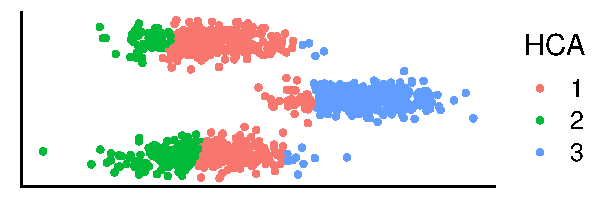
\includegraphics[width=2in]{Mahalanobis/img/hca.pdf}\quad%
	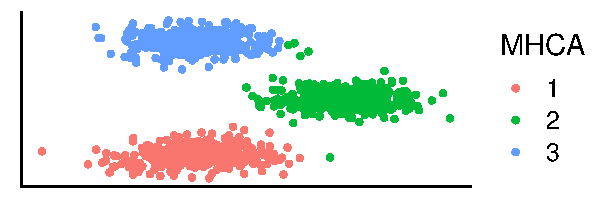
\includegraphics[width=2in]{Mahalanobis/img/mhca.pdf}
	\caption{Mahalanobis-based clustering (MHCA, right) captures the prolonged ellipsoid clusters better than commonly used hierarchical clustering (HCA, left)}
	\label{fig:mahaclust}
\end{figure}

\subsection{Contributions and Outline}

In the domain of clustering, algorithm performance has often been successfully improved by proper reimplementation for GPU hardware accelerators~\cite{krulivs2020detailed,gowanlock2017clustering,cuomo2019gpu}.
However, the computation of the MHCA is relatively irregular and rather complex, making the usual acceleration approaches ineffective.

As the main contribution of this paper, we describe our adaptation of MHCA for contemporary GPUs.
In particular, we describe a data structure that can be used to accelerate HCA algorithms on GPUs in general, and provide additional insight about efficiency of the specific parts of MHCA algorithm.
We subjected the implementation to comprehensive experimental evaluation and compared it with the existing implementation of MHCA to measure the achieved speedup.
Finally, we made the implementation available as open-source\footnote{\url{https://github.com/asmelko/gmhc}}, making it useful for both biological research and further experiments with parallelization of HCAs.

The mathematical and algorithmic overview of MHCA clustering is presented in Section~\ref{sec:mhca}, Section~\ref{sec:implementation} describes our proposed GPU implementation. We summarize the experimental evaluation in Section~\ref{sec:experiments}. Section~\ref{sec:relwork} puts the our research in proper context with prior work and Section~\ref{sec:conclusions} concludes the paper.


\section{Hierarchical Clustering with Mahalanobis Distance}\label{sec:mhca}
\label{sec:maha}

In this section, we review the necessary formalism and show the Mahalanobis average-linked hierarchical clustering algorithm.
The input dataset is a set of points in $d$-dimensional vector space, here assumed in $\mathbb{R}^d$, which is a common representation for cytometry data~\cite{shapiro2005practical}.
The algorithm produces a binary tree of \emph{clusters} where each resulting cluster is a subset of the input dataset of highly similar (`close' by some metric in the vector space) points.

Mahalanobis distance~\cite{mahalanobis1936generalized} is defined between a point $x$ and a non-singleton set of compact points $P$ as
\[ \delta_M(x,P) = \sqrt{(x-\bar{P})^T(\cov P)^{-1}(x-\bar{P})}, \]
where $\bar{P}$ is the centroid (mean) of the set $P$, and the entries of the covariance matrix are computed as
\[ (\cov P)_{ij} = \left(|P|-1\right)^{-1}\cdot \sum_{p \in P}{(p_i - \bar{P}_i)\cdot(p_j - \bar{P}_j)}. \]

One can intuitively view Mahalanobis distance as an Euclidean distance from the cluster centroid that also reflects the shape and the size of the cluster.
In particular, in a space that has been linearly transformed so that the covariance matrix of the cluster is a unit matrix, Euclidean and Mahalanobis distance coincide, as shown in Figure~\ref{fig:maha}.

\begin{figure}[t]
\centering
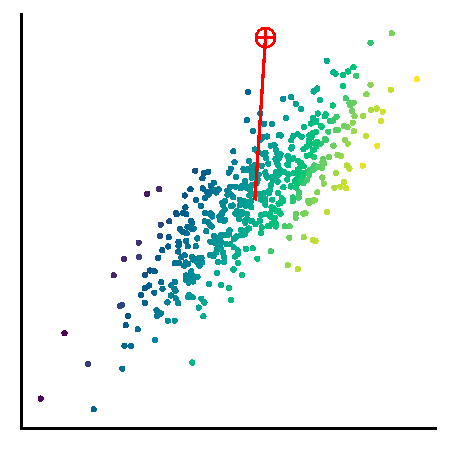
\includegraphics[width=1in]{Mahalanobis/img/maha1.pdf}\quad%
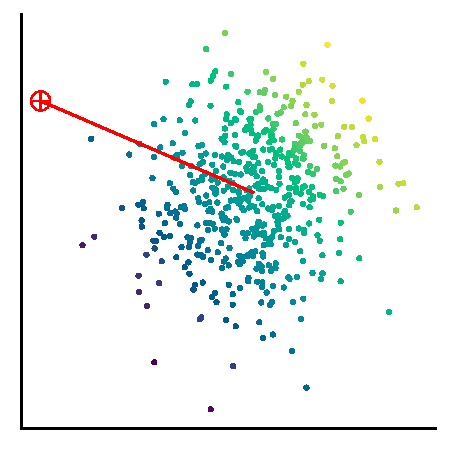
\includegraphics[width=1in]{Mahalanobis/img/maha2.pdf}
\caption{Mahalanobis distance (left) can be perceived as Euclidean distance (right) in a linearly transformed space where the cluster is perfectly `round'.
}
\label{fig:maha}
\end{figure}

The MHCA algorithm can be described in steps as follows:
\begin{enumerate}
	\item \emph{Initialization}: Construct an `active set' of numbered clusters $P_{1,2,\dots,n}$, each comprising one input element (data point) as $P_i=\{e_i\}$ for each $i \in \{1\ldots n\}$ where $\{e_1,\dots,e_n\}$ denotes the input dataset.
	\item \emph{Iteration}: Until the active set contains only a single item, repeat the following:

	\begin{enumerate}
		\item Compute pairwise dissimilarities of all clusters in $A$, select the pair $(P_r, P_s)$ with lowest dissimilarity. Output pair $(r,s)$.
		\item Update the active set by removing $P_r, P_s$ and adding $P_{n+i} = P_r\cup P_s$, where $i>0$ is an iteration number.
	\end{enumerate}

	\item \emph{Result}: the binary tree is specified by the trace of $n-1$ pairs $(r,s)$.
\end{enumerate}

Properties of the output depend mainly on the exact definition of the dissimilarity function used in step 2.a.
The common choices include the common `single' linkage (minimum pairwise distance between the 2 points in different clusters), `complete' linkage (maximum distance), `average' linkage (mean distance across clusters), `centroid' linkage (distance of cluster centroids), and others.
The used distance is usually a metric in the vector space, such as Euclidean.
The choice of the dissimilarity calculation methods is critical for obtaining results suitable for given analysis; the available methods have been therefore been subjected to much optimization~\cite{shirkhorshidi2015comparison}.

\subsection{Mahalanobis dissimilarity}

Fišer et al.~\cite{fivser2012detection} proposed the \emph{full Mahalanobis distance} as a dissimilarity function for HCA as an average of all Mahalanobis distances across clusters, as $\text{FMD}(P_i, P_j) = (|P_i|+|P_j|)^{-1} \left(\sum_k \delta_M((P_i)_k, P_j) + \sum_k\delta_M((P_j)_k, P_i)\right)$.
While this construction is intuitively correct and allows the clustering to precisely capture various dataset phenomena that are common in cytometry, the definition opens many inefficiencies and border cases that need to be resolved:

\begin{itemize}
	\item Mahalanobis distance may be undefined for small clusters because the covariance matrix is singular or nearly-singular. This can be resolved by a complete or partial fallback to robust distance measures, as detailed in Section~\ref{sec:maho-singular}.
	\item Because the Mahalanobis distance of a fixed point to a cluster \emph{decreases} when the cluster size increases (e.g., as a result of being merged with another cluster), the minimal dissimilarity selected in the step 3 of the algorithm may sometimes be smaller than the previously selected one.
  A correction is thus needed to keep the dissimilarity sequence properly monotonic, giving uncluttered, interpretable dendrogram display~\cite{everitt2002cambridge}.
	\item The amount of required computation is significantly higher than with the other linkages (dissimilarity functions), requiring additional operations for computing the inverted covariance matrix and covariance-scaled Euclidean distances.
  We mitigate this problem by massive parallelization with GPU accelerators, as detailed in Section~\ref{sec:implementation}.
\end{itemize}

The computation of the `full' average Manalanobis distance is unavoidably demanding, requiring many matrix-vector multiplications to compute distances between all points of one cluster and the opposite cluster.
Following the variations of Euclidean dissimilarity measures for HCA, a \emph{centroid-based Mahalanobis distance} may be specified to use only the average of the distance to the centroids of the other cluster, as $\text{CMD}(P_i, P_j) = \frac{1}{2} \left(\delta_M(\bar{P_i}, P_j) + \delta_M(\bar{P_j}, P_i)\right)$.
The result may be viewed as a fast approximate substitute for the full variant because the simplification removes a significant portion of the computational overhead and still produces sound results in many cases.
The difference between CMD and FMD is highly pronounced only when the centroids of the clusters are near, but their respective covariances differ, as visualized in Figure~\ref{fig:maha_var}.
Fortunately, such situations are quite rare in clustering of realistic datasets.

\begin{figure}[t]
  \centering
	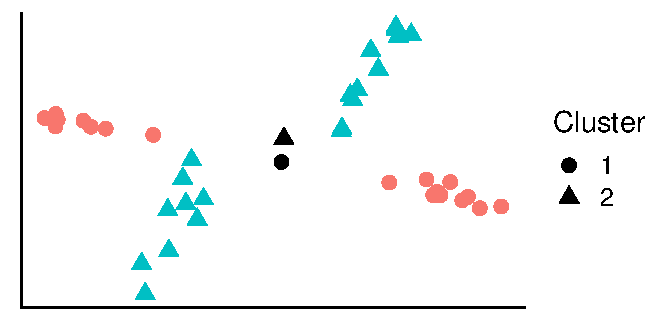
\includegraphics[width=2.2in]{Mahalanobis/img/dists.pdf}
	\caption{An example of two clusters for which the CMD fails to satisfactorily approximate the FMD (centroids are plotted in black).}
	\label{fig:maha_var}
\end{figure}

\subsection{Singularity of cluster covariance matrix}\label{sec:maho-singular}

In early iterations of MHCA, the clusters consist of only a few points.
Covariance matrix of a small cluster is likely singular, which means it is impossible to compute its inverse required by the Mahalanobis distance measure.
Furthermore, even for more points the covariance matrix may be nearly singular, and using its ill-conditioned inverse will yield inaccurate results and numeric floating-point anomalies (such as negative distances or infinities).

To solve this problem, Fišer et al.~\cite{fivser2012detection} proposed the following approach:
If the number of elements in a cluster relative to whole dataset size is lower than a threshold, the covariance matrix of such cluster is transformed so it can be inverted, and handled in a numerically safe manner.
We will denote the used threshold as the \emph{Mahalanobis threshold}, and categorize the clusters as \emph{sub-threshold} and \emph{super-threshold cluster}, depending on their size being below and above the Mahalanobis threshold respectively.

We later explore the following \emph{subthreshold handling methods} for managing the problematic covariance matrix values:
\begin{itemize}
	\item \textsc{Mahal} smoothly pushes the vectors of the covariance matrices of the sub-threshold clusters towards a unit sphere, so that the space around the clusters is not excessively distorted (or projected).
	\item \textsc{EuclidMahal} enforces unit (spherical) covariance vectors of the sub-thres\-hold clusters (thus enforcing Euclidean distances).
    Despite the simplicity and effectiveness, the hard thresholding may lead to a non-intuitive behavior; for example, the merging of a pair of large elliptical clusters that are just above the threshold may be prioritized over a pair of more similar but sub-threshold clusters.
	\item \textsc{Euclid} enforces unit covariances of all clusters \emph{only until the last sub-threshold cluster is merged}.
    This option usually leads to a viable formation of compact clusters, but completely ignores the possible intrinsic structure of several super-threshold clusters.
\end{itemize}

\subsection{Complexity and parallelization opportunities of MHCA}

A straightforward serial implementation of MHCA (such as the implementation in \texttt{mhca} R package\footnote{\url{https://rdrr.io/github/tsieger/mhca}}) works with iterative updates of the dissimilarity matrix.
Let us examine in detail the time complexity of the individual algorithm steps on a dataset that contains $n$ points of $d$ dimensions:

First, the algorithm constructs a dissimilarity matrix in $\mathcal{O}(d\cdot n^2)$, and identifies the most similar cluster pair in $\mathcal{O}(n^2)$. Then a total of $n-1$ iterations is performed as such:
\begin{itemize}
  \item a covariance matrix of the merged cluster is computed ($\mathcal{O}(d^2\cdot n)$) and inverted ($\mathcal{O}(d^3)$),
  \item the dissimilarity matrix is updated ($\mathcal{O}(d^2\cdot n)$), and
  \item the new most similar cluster pair is identified ($\mathcal{O}(n^2)$).
\end{itemize}

The total complexity is thus $\mathcal{O}(d\cdot n^2 + (n-1) \cdot (d^2\cdot n + d^3 + n^2))$.
Assuming $d\ll n$, the asymptotic complexity can be simplified to $\mathcal{O}(n^3)$.
Since we cache the unchanged dissimilarity matrix entries, the memory complexity is $\mathcal{O}(n^2)$.

In an idealized parallel execution environment (PRAM model with concurrent reads and infinite parallelism), we could improve the algorithm to perform faster as follows:
All cluster dissimilarity computations (including the later dissimilarity matrix update) can be performed in parallel in $\mathcal{O}{(d^3\cdot \log n)}$, using parallel reduction algorithm for computing the covariance sums.
The most similar cluster pair can be selected using a parallel reduction over the dissimilarity matrix in $\mathcal{O}(\log^2 n)$.
The total required time would thus be reduced to $\mathcal{O}(d^3 n\log^2 n)$ (again assuming $d\ll n$), using $\mathcal{O}(n^2)$ memory.

While this suggests two main ways of performance improvement for the massively parallel GPU implementation, the specifics of the current GPUs pose problems for such naive parallelization approach:
\begin{itemize}
	\item Parallelization of any single covariance matrix computation will improve performance only if the covariance matrix is sufficiently large, otherwise the performance may be reduced by scheduling overhead and limited parallelism.
	\item Scanning of the large dissimilarity matrix is parallelizable, but is hindered by relatively small amount of available GPU memory and insufficient memory throughput.
\end{itemize}

In the following section, we address these problems with optimizations that make the computation viable on the modern accelerators.
In particular, we show that the computation of a covariance matrix can be divided into many independent parts, thus exposing sufficient parallelization opportunities, and we demonstrate a technique for efficient caching of intermediate contents of the dissimilarity matrix to reduce the memory footprint and throughput requirements of the algorithm.

% -----------------------------------------------------------------------------
\section{GPU Implementation}\label{sec:implementation}
% -----------------------------------------------------------------------------

Memory handling optimizations form the essential part of our GPU implementation of MHCA, here called \emph{GMHC} for brevity.
Most importantly, we address the tremendous memory requirement of storing the dissimilarity matrix ($\mathcal{O}(n^2)$) for large $n$.
We replace this matrix with a special \emph{nearest-neighbor array}, which provides similar caching benefits, but requires only $\mathcal{O}(n)$ memory.
This saving in memory volume is redeemed by a slightly higher computational complexity; however, the measured improvement in scalability warrants this trade-off.

\begin{defn}[Nearest neighbor array]
	For clusters $P_1,\dots,P_n$ and a symmetric dissimilarity function $d$, the \emph{nearest neighbor array} $N$ contains $n-1$ elements defined as
	\[N_i = \argmin_{j>i} d(P_i,P_j).\]
	\label{def:nna}
\end{defn}

%(Symmetricity of $d$ is required to reduce the scope of $\argmin$ from original $j\neq i$.)

Maintaining a nearest neighbor array in the HCA computation allows us to reduce the amount of distance computations performed after each update.
In particular, when a cluster pair $(P_i,P_j)$ is merged into new cluster $P_m$, only elements with values $i$ and $j$ have to be recomputed, along with the new value for $N_m$

This is enabled by the symmetry of $d$, which allowed us to ensure that the contents of the nearest neighbor arrays at some index \emph{only depend on clusters with higher indices}.
If we set the new index $m$ to be smaller than all existing indices in the array (i.e., $m=1$, shifting the rest of the array), the newly appearing cluster can not invalidate the cached indices for the original array, and only the entries that refer to the disappearing clusters $i,j$ need to be recomputed.
In consequence, if an already present cluster $P_k$ was to form the most similar pair with the new cluster $P_m$, this information would be present the $\argmin_{k>m}$ computation, and stored in $N_m$ instead of $N_k$.

In an optimistic scenario, the above optimization can be used to limit the number of elements that need to be updated in each iteration by a constant number, which leads to a major increase in overall performance.
This constant limit is supported by empirical observations on realistic datasets with around 1 million of objects, where the number of triggered updates was rarely over $50$.
Further, we reduce the need for recomputation by caching several `nearest' neighbors for each entry of $N$:

\begin{defn}[Neighbor buffer]
A sorted list of $L$ nearest neighbor indices (respectively to the $\argmin_{j>i}$ in definition~\ref{def:nna}) stored for each item in $N$ is called a \emph{neighbor buffer}.
\end{defn}

To ensure the efficiency of the process, we split the update of neighbor buffers to two parts:
First, when $(P_i,P_j)$ is merged into $P_m$, all buffers are filtered and values $i$ and $j$ are removed (i.e, replaced with dummy values).
On recomputation, all empty buffers (including newly formed $N_m$) are filled with indices of nearest $L$ neighbors, while the partially filled buffers are left intact.
This allows us to reuse the intermediate results of the computation of an $N$ array entry for as much as $L$ recomputations that involve the cluster.

The complexity of updating the nearest neighbor array element $i$ for the neighbor buffer of size $L$ on $m$ clusters, using a pair dissimilarity computation of complexity $\mathcal{O}(\delta)$, is $\mathcal{O}((m-i)\cdot (\delta+L))$.
The reduced amount of index updates thus trades off for index update complexity, depending on $L$.
The optimal choice of $L$ is discussed later in Section~\ref{sec:exp}.

\subsection{Algorithm overview}

The hierarchical clustering of $n$ initial clusters is a series of $n-1$ iterations, such that in each iteration two clusters are merged into one. Before the first iteration, the nearest neighbor array $N$ must be initialized.
Each subsequent iteration comprises the following compact steps:
\begin{enumerate}
	\item Scan the neighbor array and fetch the most similar cluster pair
	\item Create a new cluster by merging the cluster pair
	      \subitem Compute its corresponding centroid and covariance matrix
	      \subitem Transform and invert the covariance matrix
	\item Update the neighbor array (only required if $n\geq 3$)
\end{enumerate}

\begin{figure}[t]
\centering
	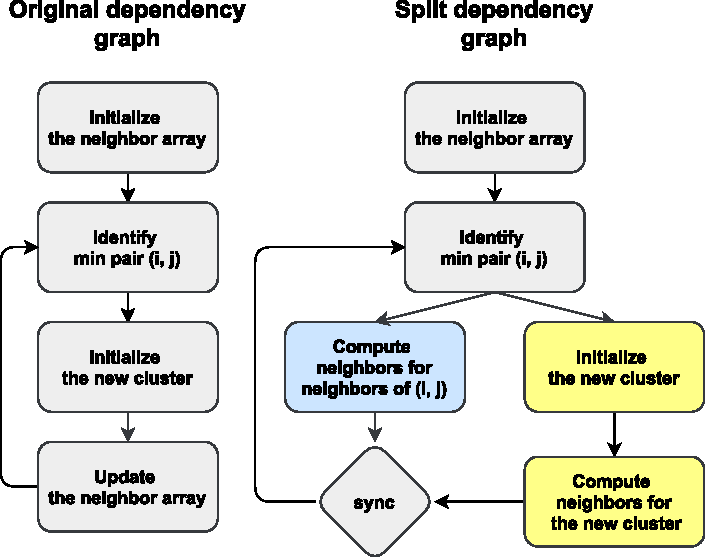
\includegraphics[width=8cm]{Mahalanobis/img/dependency-graph}
	\caption{The original graph of dependencies and the proposed split dependency graph, where blue and yellow boxes can be executed concurrently}
	\label{fig:dep-graph}
\end{figure}

The individual parts of the algorithm may be scheduled and executed dynamically, ordered only the data dependencies as displayed in Figure~\ref{fig:dep-graph}.
Mainly, this allows us to split the update of the neighbor array into update of the neighbors of old clusters ($i$, $j$) and the update of the newly created cluster.
Naturally, the individual steps are internally implemented as data-parallel operations as well.

In GMHC, we control the iteration loop from the host code, while the work of each update step is implemented within a CUDA kernel.
Our code employs CUDA streams~\cite{cuda} to efficiently implement the execution overlaps, creating some high-level task parallelism in the process.
In the rest of this section, we detail the implementations of the individual CUDA kernels.


\subsection{Cluster merging and covariance computation}

Covariance matrix $\cov P$ of cluster $P$ (and its inversion) is computed only when a cluster is formed; in our case when two clusters are merged.
In GMHC, we iterate over all data points $x \in P$ and each item $(\cov P)_{ij}$ is computed as a sum of centered products of $x_i$ and $x_j$ (following the definition from Section~\ref{sec:maha}).
As the most pressing issue, the performance of this process depends on fast finding of data points $x$ that belong to the cluster in the array of all data points.

A possible straightforward solution, storing an array of assigned points for each data cluster so that the assigned points can be accessed in a fast and compact way, would require dynamic memory allocation or manual apriori over-allocation, and many data moving operations.
We settled for a more compact solution with an assignment array that stores a cluster indices for each data point.
Although that does not require data copying, both the cluster merge and the retrieval of one cluster points will take $\mathcal{O}(n)$ time.
Fortunately, the two operations can be performed by a single parallel scan of the assignment array in this case.

\subsubsection{Covariance kernel implementation.}

The covariance kernel takes advantage of the symmetry of a covariance matrix and computes only its upper triangle.
Additionally, extra parallelism can be obtained by slicing the computation of the covariance matrix from Section~\ref{sec:maha} over individual data point contributions $\mathbf{S}^x$, as
$\cov P = (|P|-1)^{-1}\sum_{x\in P}\mathbf{S}^x$, where
$\mathbf{S}^x_{ij}=(x_i-\mathbf{\bar{x}}_i)\cdot(x_j-\mathbf{\bar{x}}_j)$.

The kernel is implemented as a loop over all data points.
A whole CUDA warp is assigned one data point and computes the intermediate $\mathbf{S}^x$.
These are then added together in a two-step reduction --- all intermediate states within a CUDA block are reduced using shared memory, which is then followed by a global reduction performed by a separate kernel launch that outputs the totals in a single covariance matrix.

Notably, the covariance matrices of single-point clusters are not computed; rather, they are assigned a default unit matrix.

\subsection{Inverse covariance storage optimization}
\label{subsec:icov}

The Mahalanobis distance requires inversion of the covariance matrix, which needs to be computed from the results of the previous step.
We use \texttt{cuSolver} library\footnote{\url{https://docs.nvidia.com/cuda/cusolver/index.html}} for implementing the matrix inversion, namely the routines \texttt{potrf} and \texttt{potri}.

The inverted matrix is subsequently transformed to better suit the Mahalanobis distance formula, and to eliminate redundant computations later in the process. In particular, we rewrite the Mahalanobis formula for inverse covariance matrix $M$ as a quadratic form
\[x^T M x =
  \sum_{i=1}^{d}\sum_{j=1}^{d}m_{ij}x_ix_j = \sum_{i=1}^{d}m_{ii}x_i^2 + \sum_{i=1}^{d}\sum_{j>i}^{d}2m_{ij}x_ix_j,\]
allowing us to store only the upper-triangular part of the matrix, pre-multiplied by $2$.

\subsection{Maintenance of nearest neighbor array}

GMHC implements 2 similar processes for the neighbor array initialization and update, differing mainly in the granularity of the task size.
We thus only focus on the update implementation.

First, specific simplified version of kernel for computing the distances is used for cases when the covariance matrix is unit, falling back to efficient implementation of Euclidean distance.
The decision which kernel to execute is done in the host code, depending solely on the selected subthreshold handling method (explained in Section~\ref{sec:maho-singular}) and the size of the two involved clusters.
The decision is formalized in Table~\ref{tab:neigh-select}.

\begin{table}[b]
	\centering
	%\setlength{\tabcolsep}{10pt}
	\begin{tabular}{@{}llll@{}}
		\toprule
		Subthreshold handling method~~ & sub/sub~~ & sub/super~~ & super/super \\
		\midrule
		\textsc{Euclid}      & \texttt{euclid} & \texttt{euclid} & \texttt{maha}  \\
		\textsc{EuclidMahal} & \texttt{euclid} & \texttt{maha}   & \texttt{maha}  \\
		\textsc{Mahal}       & \texttt{maha}   & \texttt{maha}   & \texttt{maha}  \\
		\bottomrule
	\end{tabular}
  \smallskip
	\caption{The host-side selection of the neighbor-distance kernel}
	\label{tab:neigh-select}
\end{table}


\subsubsection{The neighbor array update kernel.}

The update operation of nearest neighbor buffer array entry $N_i$ is defined as finding $L$ nearest clusters with index greater than $i$, and storing their ordered indices into $N_i$ neighbor buffer.
We split this operation in two parts, each handled by a separate kernel:
\begin{enumerate}
	\item Compute distances between all relevant cluster pairs concurrently.
	\item Reduce the results into a single nearest neighbor buffer entry.
\end{enumerate}

The execution of the first step differs between the Euclidean and the Mahalanobis neighbor computation.
While the former parallelizes trivially with one thread computing one distance value, the complex computation of Mahalanobis distance executes faster if the whole warp cooperates in one distance computation.

The precise operation needed to compute the Mahalanobis distance is a vector-matrix-vector multiplication.
To evaluate the formula from Section~\ref{subsec:icov}, we utilize the fuse-multiply-add intrinsic instructions to accumulate the results of the assigned work into their privatized buffers, which are subsequently reduced using fast warp-shuffle instructions.

In the second step, which selects the nearest $L$ indices, is the same for both distance measures.
We use a three-level implementation:
At the first level, the threads accumulate local minima of small array slices into their registers.
At the second level, each thread block utilizes the shared memory to efficiently exchange data and compute block-wise minima.
The third level collects the resulting minima and performs the same final reduction on a single thread block (thus efficiently utilizing intra-block synchronization).
The second and the third level could be fused together if the atomic instructions were used to synchronize data updates explicitly; however, we observed the improvement was negligible and preferred to reduce the design complexity instead.

This whole neighbor buffer `refill' operation is performed concurrently for every index in the nearest neighbor array that needs to be updated.
Our implementation executes a separate CUDA grid for each update, which reduces implementation complexity but still allows the grids to run concurrently and utilize the entire GPU.


% -----------------------------------------------------------------------------
\section{Experimental Results}\label{sec:experiments}
% -----------------------------------------------------------------------------

We have subjected our implementation of GMHC to extensive experimental evaluation, measuring the effect of main design choices in the algorithm.
In this section, we present the most important results and we put them in proper context, particularly with respect to parameter selection and scaling.

\subsection{Benchmarking methodology and datasets}

The experiments were performed on two systems --- a high-end server equipped with NVIDIA Tesla V100 SXM2 (32 GB) and a mainstream PC with NVIDIA GeForce GTX 980 (4 GB).
Both systems used Linux CentOS 8 with CUDA Toolkit (11.2).

We used the original MHCA clustering implementation by Fišer et al.~\cite{fivser2012detection} as a baseline, which is, to our best knowledge, the only other publicly available MHCA implementation.
The baseline algorithm is written in C as strictly sequential without explicit utilization of SIMD instructions; but it properly utilizes the highly-optimized \texttt{Blas} library for most heavy computation.
It was benchmarked on a high-end server with Intel Xeon Gold 5218 CPU, clocked at $2.3$~GHz (with 64 logical cores) and $384$~GB RAM (the same as the high-end server used for benchmarking GMHC).
We stress that the comparison between CPU and GPU implementation is not entirely objective, and the test results should be perceived more as a measure of overall data capacity improvement than of the implementation quality.
We did not test MHCA on the mainstream PC platform, because of the enormous $\mathcal{O}(n^2)$ memory requirements totaled to hundreds of gigabytes in our benchmarks.

As testing data, we used several high-dimensional datasets originating in mass cytometry~\cite{weber2016comparison}, namely the \texttt{Nilsson\_rare} (44K data points, 14 dimensions), \texttt{Levine\_32dim} (265K data points, 32 dimensions) and \texttt{Mosmann\_rare} (400k data points, 15 dimensions).
For brevity, we report only a subset of the measured results, but these should generalize well to other data.
In particular, we did not observe any significant data-dependent performance differences.

In all experiments, we measured the wall time of the total algorithm execution.
The experiments were performed multiple times to prevent random deviations in measurement; we display mean values of the measurements.
Because the experimental evaluations on both mentioned GPUs behaved consistently with no surprising differences on any particular hardware, we present mainly the results from Tesla V100 SXM2 GPU unless stated otherwise.

\subsection{Experiment results}\label{sec:exp}

First, we evaluated the scalability of the GMHC implementation depending on the size of the dataset.
The inputs of different sizes were achieved by randomly sub-sampling the Mosmann dataset.
Figure~\ref{fig:perf_methods} shows the wall time for each subthreshold method, revealing that the performance scales sub-quadratically with data size.
Notably, the optimized implementations of \textsc{Euclid} and \textsc{EuclidMahal} scale about $10\times$ better than full \textsc{Mahal} for this dimensionality.

\begin{figure}[t]
	\centering
	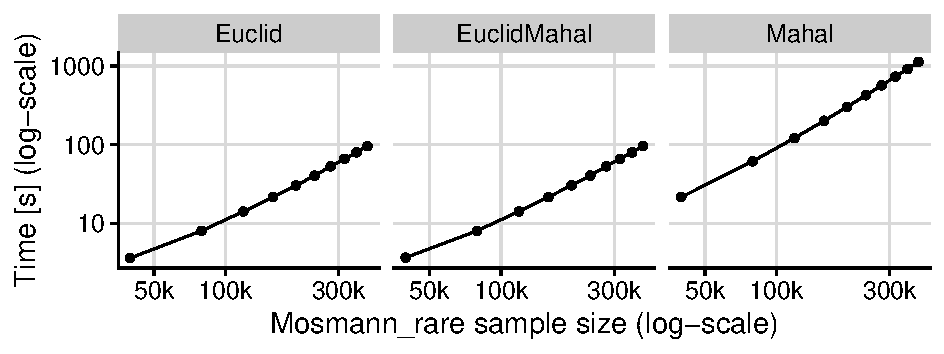
\includegraphics[width=8cm]{Mahalanobis/img/methods.pdf}
	\caption{Comparison of the subthreshold distance computation method performance.}
	\label{fig:perf_methods}
\end{figure}

The tradeoff between Euclidean and Mahalanobis computation in the first two methods can be further controlled by setting the threshold value $t$, controlling whether a cluster is considered small or large, and in turn, deciding the dissimilarity metric to use.
Figure~\ref{fig:perf_thresh} summarizes the performance gains for various setting of this threshold.

\begin{figure}[t]
	\centering
	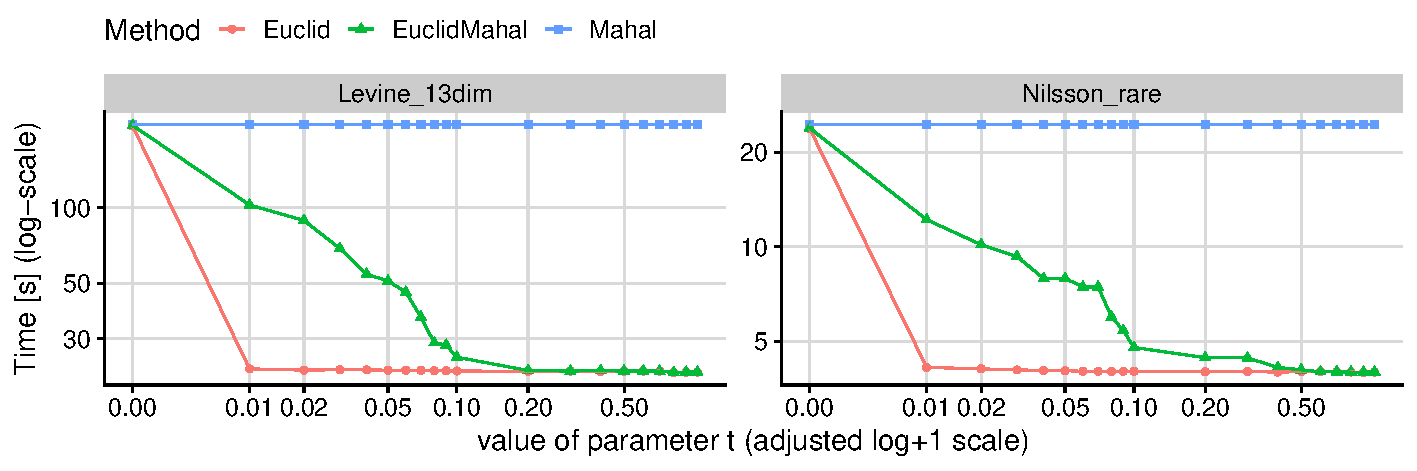
\includegraphics[width=12cm]{Mahalanobis/img/thresh.pdf}
	\caption{Clustering time of subthreshold methods with varying Mahalanobis threshold value on two different datasets.}
	\label{fig:perf_thresh}
\end{figure}

In the figure, $t=0$ forces all methods perform dissimilarity measurements using the Mahalanobis distance. When we increase $t$ only very slightly to $0.01$, the \textsc{Euclid} method time decreases dramatically and stays almost the same in the remainder of $t$ range. This is often caused by small sub-threshold clusters that are propagated to the very end of the clustering, which postpones the switch to the Mahalanobis distance. On the other hand, the \textsc{EuclidMahal} method shifts its wall time smoothly towards the \textsc{Euclid} method as $t$ increases, which is a consequence of the first super-threshold cluster appearing later in the process.

To determine the optimal value of the nearest neighbor buffer size, we benchmarked the clustering of datasets with a range of parameters $L$ (Figure~\ref{fig:perf_nei}).

\begin{figure}[t]
	\centering
	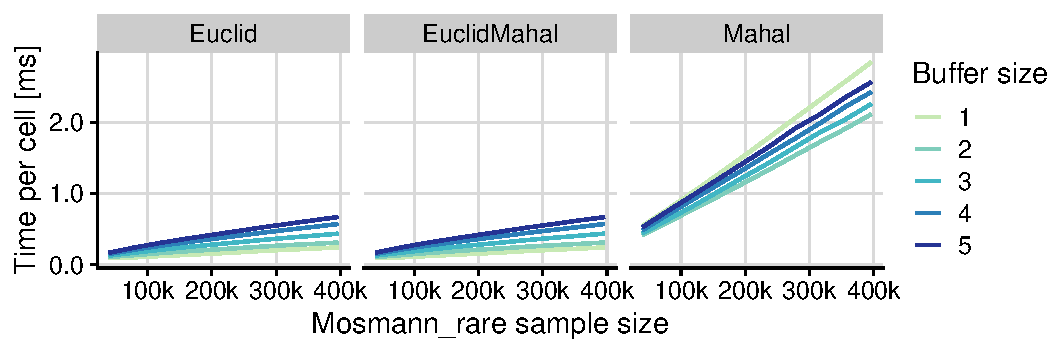
\includegraphics[width=9cm]{Mahalanobis/img/neighbors.pdf}
	\caption{Comparison of neighbor buffer sizes for subthreshold methods ($t=0.5$)}
	\label{fig:perf_nei}
\end{figure}

Curiously, the observed results show that while $L=1$ is optimal for \textsc{Euclid} and \textsc{EuclidMahal}, it performs worst for \textsc{Mahal} method. This is a consequence of the used distance function in dissimilarity measurements --- for the \textsc{Euclid} and \textsc{EuclidMahal} method, where the Euclidean distance function dominates, the time difference for performing smaller number of neighbor updates did not balance the increased time complexity of a single update. The \textsc{Mahal} method works optimally with $L=2$; as the $L$ increases further, the performance starts to decrease again. 

Similarly, the optimal value of $L$ increases for higher-dimensional datasets, which we tested on Levine\_32dim data (detailed results not shown). In particular, for Mahalanobis distance, we measured the same optimal value $L=2$ with much greater performance gain (over $30\%$) against $L=1$ than on the Mosmann dataset. We expect that the optimal value of $L$ will continue to increase with the dimensionality of the dataset in case of the \textsc{Mahal} method. On the other hand, the Euclidean-based methods kept their optimum at $L=1$.

\begin{figure}[t]
	\centering
	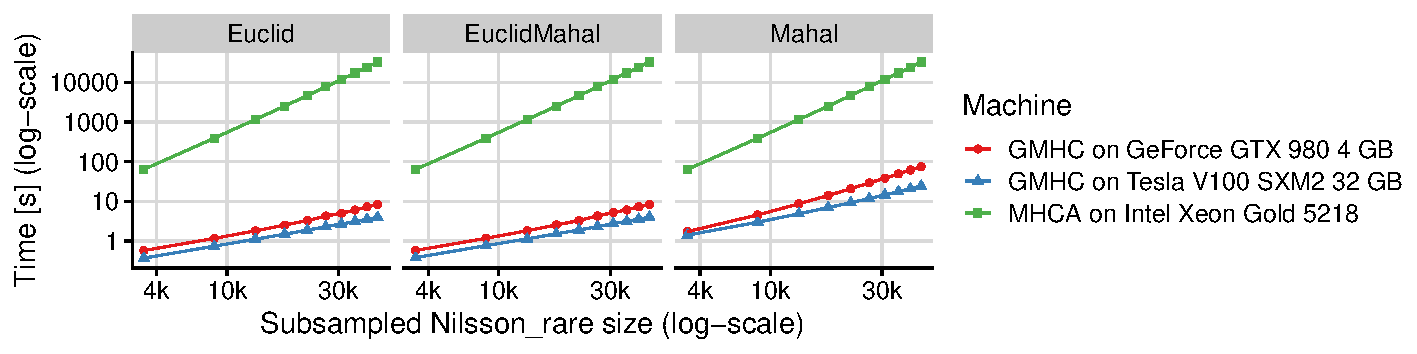
\includegraphics[width=12cm]{Mahalanobis/img/comparison.pdf}
	\caption{GMHC and MHCA comparison on Nilsson dataset with default $t=0.5$.}
	\label{fig:perf_comp}
\end{figure}

Finally, we compared the performance of GPU implementation of MHCA to the CPU baseline, to estimate the outcome for practical data analysis scalability.
Figure~\ref{fig:perf_comp}) indicates an overall performance increase by up to $1400\times$ in case of the \textsc{Mahal} method and by up to $8000\times$ in case of mixed-Euclidean methods.
When comparing performance on the older `gaming' GTX 980 GPU, the speedups were around $400\times$ and $4000\times$, respectively.
In summary, modern GPUs have been able to accelerate the MHCA task by more than three orders of magnitude, which is consistent with the effects of parallelization applied to many other clustering algorithms.


% -----------------------------------------------------------------------------
\section{Related Work}\label{sec:relwork}
% -----------------------------------------------------------------------------

The original version of MHCA clustering for flow cytometry by Fišer~et~al.~\cite{fivser2012detection} used a MATLAB implementation to analyze datasets of around $10^4$ multi-dimensional data points.
Due to the limited scalability and interoperability with modern data analysis environments, a C version of the algorithm has been implemented within R package \texttt{mhca} and enhanced with the possibility of assuming apriori clusters for approximation, to reduce the unfavorable $\mathcal{O}(n^3)$ time complexity for large datasets.
That allowed the authors to process datasets of around $10^6$ data points within an interactive environments~\cite{kratochvil2020shinysom}.

Despite of the performance advancement, the approximation in the method did not retain the sensitivity required to detect various small clusters of interest (i.e., small cell populations), such as the `minimum residual disease' cells crucial for diagnosis of acute myeloid leukemia~\cite{fivser2012detection}.
Similar approximations are used in many other clustering methods to gain performance at the cost of precision justifiable in a specific domain; including the 2-level meta-clustering approach of FlowSOM~\cite{gassen2015flowsom}, and advanced approximate neighborhood graph structure of FastPG~\cite{fastpg}.

Acceleration of HCAs on GPUs has been explored by several authors:
Chang et al.~\cite{chang2009hierarchical} discuss hierarchical clustering of gene mRNA levels assayable by DNA microarray technology.
Their GPU code computes matrix of pairwise distances between genes using Pearson correlation coefficient as one of the present metrics, and utilized a special property of data to effectively perform single-linkage over the present matrix.
Zhang et al.~\cite{zhang2006hierarchical} used similar clustering methodology, but employed GPU texture elements for the data representation of gene expression profile HCA.
Both acceleration methods resulted in performance increase between $5\times$ to $30\times$ on datasets of $10^4$ data points.


% -----------------------------------------------------------------------------
\section{Conclusions}\label{sec:conclusions}
% -----------------------------------------------------------------------------

We have presented an implementation approach for Mahalanobis-average linkage hierarchical clustering algorithm, which utilizes modern parallel GPU accelerators to increase its performance.
In the benchmarks, our GPU implementation GMHC has achieved over $10^3\times$ speedup on practical datasets over the current CPU implementations, which enabled scaling of the MHCA algorithm to large datasets produced by current data acquisition methods.

Together with the open-source implementation, we have provided a new high-performance building block for dataset analyses which should support the growing demand for fast data analysis methods not only in cytometry, but also in other areas of data analysis dealing with irregularly shaped Gaussian clusters.

The implementation structure detailed in the paper has allowed us to streamline the utilization of parallel hardware for accelerating general hierarchical clustering algorithms.
We expect that the proposed data structures will be ported to support acceleration of dissimilarity measures in other hierarchical clustering methods, providing a solid building block for future acceleration of data mining and knowledge discovery.


% \subsection*{Acknowledgements}

% This work was supported by Czech Science Foundation (GAČR) project 19-22071Y,
% by ELIXIR CZ LM2018131 (MEYS),
% by Charles University grant SVV-260451,
% and by Czech Health Research Council (AZV) [NV18-08-00385].



\chapter{Astute Approach to Handling Memory Layouts of Regular Data Structures}
% %
% \titlerunning{Handling Memory Layouts of Regular Data Structures}
% % If the paper title is too long for the running head, you can set
% % an abbreviated paper title here
% %
% \author{
%     % Anonymous\inst{1}
%     Adam Šmelko\inst{1} \and %
%     Martin Kruliš\inst{1} \and %
%     Miroslav Kratochvíl\inst{2} \and %
%     Jiří Klepl\inst{1} \and % https://orcid.org/0000-0002-2231-4073
%     Jiří Mayer\inst{1} \and % https://orcid.org/0000-0001-6503-3442
%     Petr Šimůnek\inst{1} %https://orcid.org/0000-0003-0089-7201
% }
% \authorrunning{
%     % Anonymous et al.
%     Šmelko et al.
% }
% % First names are abbreviated in the running head.
% % If there are more than two authors, 'et al.' is used.
% %
% \institute{
%     % Anonymized due to double-blind review process
%     Department of Distributed and Dependable Systems, Charles University, Prague, Czech Republic\\
%     \email{\{smelko,krulis\}@d3s.mff.cuni.cz}
%     \and
%     Luxembourg Centre for Systems Biomedicine, University of Luxembourg, Esch-sur-Alzette\\
%     \email{miroslav.kratochvil@uni.lu}
% }
% %
% \maketitle              % typeset the header of the contribution
% %
% \begin{abstract}
% Programmers of high-performance applications face many challenging aspects of contemporary hardware architectures. One of the critical aspects is the efficiency of memory operations which is affected not only by the hardware parameters such as memory throughput or cache latency but also by the data-access patterns, which may influence the utilization of the hardware, such as re-usability of the cached data or coalesced data transactions. Therefore, a performance of an algorithm can be highly impacted by the layout of its data structures or the order of data processing which may translate into a more or less optimal sequence of memory operations. These effects are even more pronounced on highly-parallel platforms, such as GPUs, which often employ specific execution models (lock-step) or memory models (shared memory).

% In this work, we propose a modern, astute approach for managing and implementing memory layouts with first-class structures that is very efficient and straightforward. This approach was implemented in \Noarr{}, a GPU-ready portable C++ library that utilizes generic programming, functional design, and compile-time computations to allow the programmer to specify and compose data structure layouts declaratively while minimizing the indexing and coding overhead. We describe the main principles on code examples and present a performance evaluation that verifies our claims regarding its efficiency.
% \keywords{memory layout \and data structure \and cache \and parallel \and performance \and reusable}
% \end{abstract}

% -----------------------------------------------------------------------------
\section{Introduction}
% -----------------------------------------------------------------------------

This paper aims to tackle memory-related performance issues, which represent one of the most crucial performance optimization topics. In hardware, memory access is optimized by providing faster memories closer to the chip (like HBM2), multi-level caches and transfer buffers, and even specialized explicit near-core memories (such as AVX512 registers or shared memory in Nvidia GPUs). Software developers benefit from these features by creating specialized, cache-aware algorithms, often tailored for a particular architecture.

The design of the way that the program data is laid out in memory is one of the crucial steps that ensures memory access performance. Even simple design choices like row- or column-major matrix storage impact the performance within the complex memory cache models by simplifying address translations, improving cache hit ratio and prefetching, or ensuring the alignment required for coalesced SIMD operations~\cite{clauss2000automatic,panda2001cache}. For parallel algorithms, the complexity of the problem becomes much broader because of cache-line collisions, false-sharing, non-uniform memory architectures, a variety of synchronization issues~\cite{bethel2015improving,heinecke2008parallel,weidendorfer2007latencies}, and other factors. Many-core platforms (GPUs in particular) only amplify this by enforcing specific data access patterns in lockstep execution, advocating the use of programmer-managed caches (like shared memory), and having a significantly lower cache-to-core ratio in comparison to the CPUs~\cite{guide2013cuda}.

The best layout is quite often elusive and needs to be discovered empirically. Furthermore, it often differs even among the utilized cache levels~\cite{weber2017matog,hawick2011hypercubic,krulivs2020detailed}. Consequently, the optimal implementations are often complicated, and most of the optimization-relevant code is not portable between hardware architectures. Enabling simple implementations of layout-flexible data structures and algorithms would improve the code portability (and value); however, systematic approaches are quite rare, often over-complicating the code logic and making the algorithm implementation not maintainable or usable beyond the community of specialists.


\subsection{Motivational example}

To explain the motivation, objectives, and contributions of our research, we have selected a matrix multiplication problem widely known in computer science. For the sake of simplicity, we use the most straightforward implementation with $\mathcal{O}(N^3)$ complexity (computing $C = A \times B$ of square matrices $N^2$):

\begin{minted}[fontsize=\scriptsize]{c++}
    for (size_t i = 0; i < N; ++i)
        for (size_t j = 0; j < N; ++j) {
            C[i][j] = 0;
            for (size_t k = 0; k < N; ++k)
                C[i][j] += A[i][k] * B[k][j];
        }
\end{minted}

Having a fixed algorithm structure (i.e., order of the operations), the memory layout of the matrices is the main issue affecting the performance. In this context, the layout is defined by transforming the abstract indices ($i,j$) into an offset, subsequently used to compute the actual memory address. For instance, the most common matrix layout is row-major, which computes the offset as $i*W + j$ (where $W$ is the width of the matrix). A few examples of possible layouts are depicted in Figure~\ref{fig:layout}.

\begin{figure}
    \begin{subfigure}{.19\textwidth}
        \centering
        \includegraphics[width=.9\linewidth]{noarr/figures/matrix-row-major}
        \caption{row-major}
        \label{fig:layout-row}
    \end{subfigure} 
    \begin{subfigure}{.19\textwidth}
        \centering
        \includegraphics[width=.9\linewidth]{noarr/figures/matrix-col-major}
        \caption{col-major}
        \label{fig:layout-col}
    \end{subfigure}
    \begin{subfigure}{.19\textwidth}
        \centering
        \includegraphics[width=.9\linewidth]{noarr/figures/matrix-tiled}
        \caption{row-tiles}
        \label{fig:layout-tile}
    \end{subfigure}
    \begin{subfigure}{.19\textwidth}
        \centering
        \includegraphics[width=.9\linewidth]{noarr/figures/matrix-zcurve}
        \caption{z-curve}
        \label{fig:layout-zcurve}
    \end{subfigure}
    \begin{subfigure}{.19\textwidth}
        \centering
        \includegraphics[width=.9\linewidth]{noarr/figures/matrix-hcurve}
        \caption{Hilbert curve}
        \label{fig:layout-hcurve}
    \end{subfigure}
    
    \caption{Examples of common matrix layouts}
    \label{fig:layout}
    \vspace{-10pt}
\end{figure}

The aforementioned code sample used traditional C notation \mintinline{c++}{A[i][j]} which enforces the row-major layout, which is sub-optimal for this algorithm. Having the second matrix in a col-major layout or using a z-curve for all matrices will improve cache utilization, and the algorithm would run several times to several orders of magnitude faster, depending on the platform. Therefore, we need to introduce layout flexibility into the code.

A typical object-oriented solution would be to create a class abstraction that would define a uniform interface for accessing matrix elements whilst enabling different implementations through derived classes. A slightly better and more reusable solution would be to separate the offset computation into a policy class that would be injected into the matrix as a template parameter:

\begin{minted}[fontsize=\scriptsize]{c++}
    class RowMajor {
        static size_t offset(size_t i, size_t j, size_t W, size_t H) {
            return i*W + j;  
        }
    };

    template<typename T = float, class Layout = RowMajor>
    class Matrix {
        /* ... */
        T& at(size_t i, size_t j) {
            return _data[Layout::offset(i, j, _W, _H)];
        }
    };
\end{minted}
  
The policy class makes the matrix implementation flexible (in terms of selecting the proper layout) and efficient (since the compiler can inline the static method). However, several drawbacks make this solution imperfect. The interface between the \texttt{Matrix} class and its layout policy (\texttt{RowMajor}) is created ad-hoc by the author of the main class, which complicates the code reusability of the layout policies in potentially compatible situations. The interface also prevents efficient constant propagation and caching of intermediate values. Furthermore, the strong encapsulation may prevent low-level optimizations, portability to other architectures (e.g., GPUs), and complicate data structure composition (e.g., when matrices in an array need to be interleaved).

We aim to design a more straightforward, more programmer-friendly solution to implementing \emph{layout-agnostic} algorithms, focusing on enabling performance optimizations and parallel processing.


\subsection{Objectives and contributions}

Our main objective was to create a library that allows the users to quickly adapt their algorithms and data structures for different memory layouts, with a~particular focus on the following targets:

\begin{itemize}
    \item Once an algorithm is adapted, it becomes layout-agnostic --- i.e., no subsequent internal code modifications should be required to change the layout of the underlying data structures.
    \item The layout representation should not be coupled with memory allocation so that it could be used in different scenarios and different memory spaces (i.e., directly applicable with memory-mapped files or GPU unified memory).
    \item The interface should define an easily comprehensible abstraction for \emph{indexing} (offset computation) that would hide its (possibly complex) nuances.
    \item The indexing mechanism should enable the compiler to evaluate constant expressions at compile time (e.g., fold constant dimensions of a structure into the generated code).
    \item The code overhead should be minimal, preferably smaller than with well-established practices, such as providing template policy classes to govern layout or allocation.
\end{itemize}

We have implemented \Noarr{} header-only library\footnote{\Noarr{} is available as open-source on GitHub under MIT license: \url{https://github.com/ParaCoToUl/noarr-structures}} for C++ as a prototype that achieves the outlined objectives. C++ was chosen as a widely-used mainstream language that provides complete control over memory layout and allocation and is widely used for programming performance-critical applications, including parallel HPC systems and GPGPU computing. Its fundamental features, like the templating system and operator overloading, open possibilities for generic programming, compile-time optimizations, and the design of a functional-like interface, which simplifies the use of the library. Furthermore, the separation of indexing from (CPU-specific) memory management allowed us to directly utilize the library with Nvidia CUDA code, easily porting the layout-agnostic code on contemporary GPUs.

We believe that \Noarr{} will make a significant contribution to simplifying the coding process and increasing performance in many scenarios, especially:
\begin{itemize}
    \item Empirical exploration of possible layouts --- i.e., finding the optimal combination of layouts for given data structures and algorithms by measuring the performance of all possible implementations.
    \item Implementing applications and libraries in which the optimal layout of data structures needs to be selected at runtime (e.g., based on the size of the problem or the best available architecture).
    \item Allowing simple yet efficient (semi)automatic layout transformations in case the input or output layouts differ from the optimal layouts for the computation.
\end{itemize}

Although the issues mentioned above can be identified in a large variety of data structures and algorithms, we are focusing mainly on regular data structures such as nested multi-dimensional arrays and structures (in the C/C++ sense). However, despite this narrow scope, we have identified that this problem is quite challenging, especially regarding optimizations for massively parallel environments like GPUs.

% Furthermore, \Noarr{} library enables research of semi-automated or automated selection of the best memory layout for given problem configuration, and automatic layout transformations of data structures that are often required when moving the data between memory types (e.g., when a row-major matrix from disk is transferred to a column-major format in memory). Here, we mainly demonstrate the possibility of automating the layout transformation process. Although the automated selection of the best data layouts for algorithms is easy to implement with the current version of \Noarr{}, a rigorous review of the methodology is well beyond the scope of this paper.


The paper is organized as follows. Section~\ref{sec:layouts} explains the key principles and benefits of the layout-agnostic algorithm design. The performance aspects of offset computation overhead are summarized in Section~\ref{sec:perf}. In Section~\ref{sec:implementation}, we provide insights into the current implementation of the \Noarr{} library. Related work and main conclusions are summarized in Sections~\ref{sec:relwork} and \ref{sec:conclusion}.

%\section{Motivational Example}\label{sec:motivation}

To demonstrate both performance- and programming-related aspects of the data layout reorganization, we selected a matrix data structure, which is well-known by all scientists and programmers. Matrix is two-dimensional regular array where the individual elements are simple scalars (e.g., floats) and there are many ways how it can be stored in linear memory.

The two most typical layouts are the \emph{row-major} and \emph{column-major} formats, where the items in each row (or column, respectively) form a continuous sequence. The memory offset of item at position $[i,j]$ is computed as $i\cdot W + j$ in row-major layout, and $j*H + i$ in column-major layout, where $i$ is a zero-based index of the row, $j$ is the index of the column, and $W,H$ stand for the width and the height of the matrix respectively.

\begin{figure}
\begin{subfigure}{.19\textwidth}
    \centering
    \includegraphics[width=.9\linewidth]{figures/matrix-row-major}
    \caption{row-major}
    \label{fig:layout-row}
\end{subfigure} 
\begin{subfigure}{.19\textwidth}
    \centering
    \includegraphics[width=.9\linewidth]{figures/matrix-col-major}
    \caption{col-major}
    \label{fig:layout-col}
\end{subfigure}
\begin{subfigure}{.19\textwidth}
    \centering
    \includegraphics[width=.9\linewidth]{figures/matrix-tiled}
    \caption{row-tiles}
    \label{fig:layout-tile}
\end{subfigure}
\begin{subfigure}{.19\textwidth}
    \centering
    \includegraphics[width=.9\linewidth]{figures/matrix-zcurve}
    \caption{z-curve}
    \label{fig:layout-zcurve}
\end{subfigure}
\begin{subfigure}{.19\textwidth}
    \centering
    \includegraphics[width=.9\linewidth]{figures/matrix-hcurve}
    \caption{Hilbert curve}
    \label{fig:layout-hcurve}
\end{subfigure}

\caption{Examples of common matrix layouts}
\label{fig:layout}
\end{figure}

More elaborate matrix storage layouts may promote 2D locality of the data. For instance, a matrix can be divided in tiles of $T_w \times T_h$ elements\footnote{For the sake of simplicity, we are not covering the details of handling matrix sizes that are not divisible by tile sizes.}, which are each stored as a compact block. Both the tiles and the elements within a tile may use row-major or column-major layout independently, and the tiling division can be employed on multiple levels. Ultimately, recursive subdivision leads to patterns such as the z-order curve or Hilbert curve~\cite{dai2003locality}. Examples of possible layouts are illustrated in Figure~\ref{fig:layout}.


% -----------------------------------------------------------------------------
\subsection{Performance aspects of matrix layout}\label{sec:motivation-perf}
% -----------------------------------------------------------------------------

The memory layout in combination with a particular algorithm implementation determines a memory access pattern. Different access patterns may have different performance characteristics due to properties of the selected hardware platform. The most important ones comprise:

\begin{itemize}
    \item \textbf{Hardware caches} are integral part of memory architectures, reduce the main memory latencies that are orders of magnitude higher than the latency of the registers or closest-level of caches. The optimization of their performance usually aims to minimize the amount of loads of cache lines (fixed-size cache units) from the main memory. Equivalently, programmers may aim to minimize the amount of unneeded data loaded with each cache-line by close positioning the data elements required at the same time.
    \item \textbf{Prefetching} speeds up data loading in cases when the CPU is able to detect the location of a memory access in advance, and start fetching the data before these are actually required. Most CPUs are able to reliably detect a simple sequential access pattern.
    \item \textbf{Virtual address translation} is performed with every memory access, requiring lookup in page table addresses. To speed up the lookup, a fast TLB is used as a cache. TLB misses may start to affect the performance in case a typical size of a TLB (usually hundreds of items at most) is exceeded by the amount of `active' memory pages.
\end{itemize}

In consequence, a straightforward single-pass sequential access typically yields optimal performance characteristics, conversely a completely random access pattern over large chunk of memory will prevent function of the caches and prefetching mechanism, leading to poor performance. For demonstration, we show the effects on the example of matrices, using a na\"{i}ve transpose algorithm of a square matrix impact. The algorithm might be implemented as follows:

\begin{minted}[fontsize=\scriptsize]{c++}
  for (size_t i = 0; i < N; ++i) {
    for (size_t j = i+1; j < N; ++j) {
      std::swap(m[i][j], m[j][i]);
    }
  }
\end{minted}

We can observe that both row-major and column-major layouts would be suboptimal for sufficiently large matrices. In each step, two items from the matrix are swapped. In row-major layout, the first arguments for swap (\texttt{m[i][j]}) will be accessed in optimal sequential manner, but the second ones (\texttt{m[j][i]}) will exhibit a highly strided access (two subsequent accesses are $N$ items apart) which may not be detected by prefetcher and may cause `cache spilling', as each data item is loaded with entire cache line.

Employing a z-order curve layout will mitigate the difference between row-first and column-first access, especially from the perspective of cache utilization. The row-first access pattern is only slightly worse than with the row-major layout but the column-first access is improved significantly. As a result, the algorithm may run several times to several orders of magnitude faster, depending on the platform.

Alternatively, one may utilize a different algorithm for matrix transpose. A fast approach designed for contemporary architectures is based on recursive decomposition of the matrix, where each step divides the given sub-matrix into four quadrants and transposes them in sequence. The effect on data access pattern is similar to selecting an optimal layout for the sequential algorithm, which comes at the cost of making the algorithm implementation more complex and potentially error prone.

For this reason, here we mainly aim to change the layouts of the underlying data structures, while keeping the algorithm intact in its most apprehensible form.


% -----------------------------------------------------------------------------
\subsection{Decoupling layouts from algorithms}
% -----------------------------------------------------------------------------

To make the algorithms adaptable to many layouts, we need to programmatically abstract out the implementation of all layout-specific computation, with a uniform, layout- and algorithm-agnostic interface. With matrices, we may require a method that returns a reference to an item based on $i,j$ coordinates.

In a traditional OOP-design, a matrix would be encapsulated in an object where the item accessor would be a method:
\begin{minted}[fontsize=\scriptsize]{c++}
  template<typename T = float> class Matrix {
  public:
    T& at(size_t i, size_t j) { /* ... */ }
  };
\end{minted}

For implementing different layouts, programmer might choose to inherit the methods into the class. However, that would require \texttt{at()} to be a virtual method, requiring to perform late binding upon each data item access, which is sub-optimal from the performance point of view.

A more elaborate, frequently used approach is to introduce a~policy class that governs the layout (and possibly other concerns, including memory allocation), and parametrize the matrix wrapper:

\begin{minted}[fontsize=\scriptsize]{c++}
  class RowMajor {
    static size_t offset(size_t i, size_t j, size_t W, size_t H) {
      return i*W + j;  
    }
  };

  template<typename T = float, class Layout = RowMajor>
  class Matrix {
    /* ... */
    T& at(size_t i, size_t j) {
      return _data[Layout::offset(i, j, _W, _H)];
    }
  };
\end{minted}

The policy class makes the matrix implementation both flexible (in the terms of selecting proper layout) and efficient (since the static method can be inlined by the compiler). However, several drawbacks make this solution imperfect:

\begin{itemize}
    \item The interface between the main class (i.e., \texttt{Matrix} in the previous example) and its layout policy (\texttt{RowMajor}) is created ad-hoc and is typically designed by the author of the main class. That complicates code reusability of the layout policies in potentially compatible situations (e.g., when matrix layout needs to be adopted for a structure that represents vector of points in $\mathbb{R}^d$).
    \item The interface often prevents efficient constant propagation and caching of intermediate values. For instance, the size of the matrix is passed down to \texttt{offset()} at each call, which may be suboptimal if the dimensions are compile-time constants and inter-procedural optimization is not admissible. Furthermore, accesses to items of one row in row-major layout may require unneeded repetitive re-computation of $i\cdot W$ since the policy can not predict the access pattern, and the main class cannot make any assumptions about the layout.
    \item The strong encapsulation of the data in class \texttt{Matrix}, which is considered a good-practice in general, may hinder the optimization efforts employed in performance-oriented programming. The class and algorithms that use it cannot be easily ported to GPU architectures for instance, and impose a data interface that may be detrimental for certain more complex access methods (such as block-wise loads with SIMD or offloading parts of the matrix to shared memory of a GPU).
    \item The encapsulation provided by the main class also complicates integration in larger data structures. For example, a collection of matrices may benefit from a memory layout where the matrices are interleaved.
\end{itemize}

% -----------------------------------------------------------------------------
\subsection{First-class indexing structures}
\label{subsec:fstclass}
% -----------------------------------------------------------------------------

\begin{listing}[h]
    \vspace{-10pt}
    \inputmintedcpp{noarr/code-snippets/noarr_transpose.cpp}
    \vspace{-20pt}
    \caption{The example of matrix transpose that employs first-class layout structures implemented in \Noarr{} library.}
    \label{lst:demo-noarr}
\end{listing}

To improve upon the drawbacks mentioned in previous section, we introduce layouts as first-class structures, which provide the required indexing (offset computation) operations, expose the details of the layout to the programs, and can be easily composed to form complex layouts from smaller primitive `building blocks' having the type of the layout flexible and easily constructible from pre-implemented primitives. The main features are demonstrated in Listing~\ref{lst:demo-noarr}, which shows the matrix transpose algorithm implemented with the first-class layout structures.

In the example, the layout type (row-major in this case) is constructed on line $30$ from the \Noarr{} primitives for vectors of items. These are connected to a sequence of matrices on line $31$. The structure has explicitly named dimensions, here marked with characters\footnote{Any type convertible to integer can be used for dimension names, including enumerations.}, which makes the access more mnemonic for the programmers (as seen on line $5$). The naming of the dimensions is entirely processed at compile-time by the C++ compiler, creating no overhead in the resulting code.

The matrix sequence layout object is created on line $33$ to provide dynamic sizes to a statically defined layout type. This is achieved by instantiating \texttt{matrix\_sequence} type and by applying \texttt{set\_length} functions to each dimension specified by a character literal. On line $37$, the layout object is converted into a \texttt{bag} structure that, for convenience, explicitly binds the layout and a data pointer together, creating a work-alike of common data objects. The actual allocation of the memory is not shown in the example, but may be executed by a helper function that determines the required size from the layout object. Line $37$ demonstrates a `partial' indexing, fixing arbitrary dimensions of the layout structure, so that the \texttt{transpose()} function can only work with a single pre-selected matrix. This corresponds to creation of arbitrary (even irregular) array slices.

The structure object is passed to functions in two parts --- as a value (first-class parameter) and also as type (template parameter). This way, both static data (such as the size and type of the `scalar' contents, and static sizes of arrays) and dynamic data (sizes of the vectors) are visible to a compiler.

The layout structure provides additional methods to help with various indexing scenarios. For instance, the \texttt{shift} method (lines 24 and 25) creates a copy of the layout structure with shifted origin (i.e., with explicit offsets embedded), simplifying the implementation of divide-and-conquer recursive pattern used in the transpose algorithm. The explicit dereferencing of the \texttt{bag} structure (the \texttt{at} method at line 5) combines computation of the offset from the layout and adding the offset to the stored pointer.

In the following sections, we detail the implementation and analyze the key benefits of this approach.

\section{Extensible Memory Layout Structures}\label{sec:layouts}

One of the most significant challenges of the outlined problem is to create an indexing abstraction that would follow the fundamental code design principles (especially in object-oriented programming, which is one of the most widely adopted paradigms), thus allowing the programmer to write neat and maintainable code, whilst minimizing performance overhead and making heavy use of the compile-time optimizations.

In this work, we propose using first-class indexing structures which can be detached entirely from the allocated memory and the data structures themselves. The indexing structure has a specific type (templated class) composed of predefined base types and a corresponding instance (object). This way, the information being passed to the layout-agnostic algorithm is divided into two parts:
\begin{itemize}
\item the data type passed via (inferred) template parameter, which bears the structure and constant parameters,
\item and the object, which bears all dynamic parameters (such as sizes of non-constant dimensions of the data structure).
\end{itemize}

Before we focus on the benefits, let us emphasize the C++ cornerstones of \Noarr{} that are pretty important for understanding the main principles (details are provided in Section~\ref{sec:implementation}).

\begin{itemize}
    \item The indexing structure type composition is straightforward as the user merely combines predefined \Noarr{} templated classes. Furthermore, thanks to the templating system, it is easy to create partially-defined structures, thus promoting code reusability. The construction of derived or augmented types (like binding the constant dimensions) is implemented in a functional manner, which is quite comprehensive and easy to write. Finally, modern C++ constructs like \mintinline{c++}{auto} or template type inference make these type modifications easier to handle since only the instance object is passed down.
    \item The dimensions of the data structure are denoted using chars (typically letters), which are much more mnemonic than numbers or the order of definition. Furthermore, they can be used to define additional abstraction so that structures with the same set of named dimensions can be treated as compatible, regardless of the order of their definition or their actual layout representation.
    \item Finally, the implementation makes heavy use of \mintinline{c++}{constexpr} functions which allow the compiler to be inlined, resolve, and even precompute many pieces of the layout-related code, thus making it more efficient. For instance, the constant dimensions can be translated into the expressions where the actual memory offsets are being computed, which may allow optimizations like precomputing constant subexpressions.
\end{itemize}

Utilizing memory layouts as first-class objects can introduce some flexibility into the code. In this section, we demonstrate the two main ideas of the proposed approach: The ability to easily \emph{decouple memory allocation from its interpreted layout} and the possibility of writing \emph{memory-layout-agnostic functions}. Listing~\ref{lst:matmul} presents an example that employs both these ideas using \Noarr{} library.

% There are two traditional approaches to the problem. The most straightforward design is to have an abstract class that encapsulates a data structure and derived classes for individual implementations. Unfortunately, this approach often offers minimal opportunities for code reusability and requires dynamic code selection (typically implemented by method late binding), creating unacceptable overhead in high-performance applications.

% The second approach takes advantage of C++ templating and policy classes. A data structure layout (i.e., the indexing algorithm) can be implemented in a policy class that is given the data structure class as a template argument. This will provide some reusability, and the compiler can perform many optimizations due to method inlining. However, if the layout requires dynamically specified parameters (e.g., a size of a dynamically allocated array), these parameters must be stored in the data-structure class, and the layout policy must somehow access it, which creates several complications.

%We will explain this concept in the following examples that explain its applicability in various situations.

% -----------------------------------------------------------------------------
\subsection{Decoupling the memory management}
% -----------------------------------------------------------------------------

\begin{listing}
    \vspace{-10pt}
    \inputmintedcpp{noarr/code-snippets/matmul_tile.cu}
    \caption{CUDA matrix multiplication kernel based on \Noarr{} library}
	\vspace{-20pt}
    \label{lst:matmul}
\end{listing}

In C++, memory is usually acquired following one of two scenarios --- either it is allocated internally by a wrapping data structure (the `owning' semantics), or it is provided by the caller (the `borrowing' semantics). When the indexing structure is decoupled from the memory allocation and combined with the borrowing semantics, it can cover many elaborate memory management scenarios, such as file memory-mapping or sharing memory among threads (this also includes CUDA unified memory or shared memory).

In \Noarr{}, the layout objects are entirely independent of memory management. To simplify the situation for programmers, it also provides a wrapper structure \texttt{bag}, which binds the layout structure with any pointer, acting as a smart pointer with borrowing semantics. The layout can be used alone to compute linearized offsets from input indices, which is also applicable in hypothetical scenarios beyond pointer-based memory addressing.

We present an example of a matrix multiplication kernel implemented in CUDA (Listing~\ref{lst:matmul}) to demonstrate the possibilities opened by proper decoupling. In the code, a GPU kernel performs the multiplication in tiles where each $16\times16$ tile of the output matrix is computed by one thread block, and each element is handled by one thread. A thread block cooperatively fetches a pair of tiles from the input matrices (one pair at a time) into the shared memory; all threads of the block then use the cached tiles to update their intermediate scalar products (which are kept in their registers) before iteratively loading successive pairs of tiles. Once all tiles are processed, each thread writes its aggregated result into the output matrix.

The example focuses on a typical pattern in GPU programming --- a manual caching of data in the \emph{shared memory}. Unlike global memory (accessible by all threads), the shared memory is an integral component of a streaming multiprocessor; thus, it is dedicated to the threads within the same thread block. Unsurprisingly, the two types of memory are allocated and managed in slightly different ways, albeit both use pointer-based addressing. The global memory is usually allocated before the execution of a kernel (i.e., by the host) and passed to a kernel as an argument (\texttt{lhs\_in}, \texttt{rhs\_in}, and \texttt{out} on line $2$ of Listing~\ref{lst:matmul}). The shared memory is acquired inside the kernel by defining a C array with \texttt{\_\_shared\_\_} prefix (\texttt{l\_tile} and \texttt{r\_tile} on lines $5$--$6$).

Considering also the host memory (where a copy of matrices also needs to reside), the programmer must manage three (partial) copies in three different memory spaces. A uniform abstraction (that supports owning and borrowing semantics) streamlines the code significantly. Furthermore, in this particular instance, we could also take advantage of having a different layout for different matrices --- e.g., the optimum is reached if the left-side matrix is in the row-major while the right-side matrix is in the column-major format.
% The matrix data may be additionally stored in host memory, which is allocated with the usual means (such as \texttt{malloc}). If the programmer requires to use the same layout description for all 3 memory types, the layout abstraction is inevitably required to operate independently on memory space, and support both owning and borrowing semantics (for global and shared memory allocations, respectively). To add complexity to the task, all input and output matrices and cache layers may require different layouts (for example, left-hand side is slightly better stored in row-major format if the right-hand side is column-major).

% Now, let us introduce an idea that instead of implicitly expecting an a priori structure that each allocated piece of memory has, we explicitly specify the structure in a programmatic way. To do so properly, we need to take into account the complex memory management of GPU devices. The simplest option is to represent the memory layout as a C++ policy class. This has a clear downside because the whole memory structure is coded just into a class type (rather than an object), and, as it can not be dynamically instantiated, the trivial task of selecting the dimension size would be infeasible. Solving the disadvantage of this approach is simple; having the memory layout represented in an instantiated object.

% This approach can be taken two ways, the most simple one being a single instantiable class that encompasses all the work with a piece of memory --- the allocation, layout definition, indexing, etc.. As this may seem usable in theory, the implementation would suffer from the need of including all the allocation possibilities, which would become easily unsustainable with the support for GPU devices. Also including the specification of custom memory layout, the number of instantiation possibilities becomes enormous. For this reason, it is logical to decouple the memory allocation from the memory layout and design an instantiable class that represents only the latter.

Listing \ref{lst:matmul} demonstrates, how the problem is solved using \Noarr{}. The tiles are loaded into the shared memory on lines $12$--$15$. The variables \texttt{lhs\_s} and \texttt{rhs\_s} represent the layout objects, which are bound with global memory pointers (\texttt{lhs\_in} and \texttt{rhs\_in} respectively) to read data from input matrices (lines $13$ and $15$). Another layout object \texttt{tile\_s} is used for two shared memory pointers representing the cached tiles (lines $12$ and $14$).
With these layout objects, different types of memory could be accessed using the same interface. Additionally, the code is ready for future layouts modifications and promotes the reusability of the existing layout structures.


% -----------------------------------------------------------------------------
\subsection{Layout-agnostic functions}\label{sec:layouts-agnostic}
% -----------------------------------------------------------------------------

Formally, we may define the layout-agnostic property as a unique form of polymorphism. Layout-agnostic functions are implemented in a way that does not require altering their code when the layout of the used data structures needs to be changed. As hinted in the introduction, the layout selection may significantly affect performance. In extreme cases, the relative performance improvement achieved by optimal layout selection can reach orders of magnitude.

To demonstrate this effect, we show how the layout choice changes the performance of the matrix multiplication kernel from Listing \ref{lst:matmul}, which is already written as layout-agnostic. Running the kernel with different layout configurations for each matrix is implemented by simply passing different function arguments (and corresponding template parameters, which the compiler can automatically infer in typical cases). We utilize this flexibility to find a layout combination that exhibits the best performance quickly.

For the sake of this example, we coded the following matrix layouts:
\begin{itemize}
    \item \emph{Row-major} layout (labeled \textbf{R}, which we use as a baseline)
    \item \emph{Column-major} (\textbf{C}, a transposition of row-major layout)
    \item \emph{\textbf{R} tiles in \textbf{C} order} (\textbf{RC}), which divides the matrix logically into $16\times16$ sub-matrices (tiles); data in each sub-matrix is stored with row-major layout, while the sub-matrices are organized in column-major layout
    \item \emph{\textbf{C} tiles in \textbf{R} order} (\textbf{CR}) is analogical to \textbf{RC} layout, but the tiles use column-major layout internally, and are ordered in row-major fashion
    \item \emph{\textbf{CC}} and \emph{\textbf{RR}} are defined analogically
\end{itemize}

The layout of all inputs and outputs of the matrix multiplication is thus expressed as a triplet of individual matrix layouts. For example, $\textbf{R}\times \textbf{C}=\textbf{R}$ denotes a multiplication where the left and the output matrices are in row-major, and the right-side input matrix is in the column-major layout. Since the kernel \ref{lst:matmul} already caches tiles explicitly in the shared memory, we expect the tiled layouts to perform better. Likely, the $\textbf{RR}\times\textbf{RC}=\textbf{R}$ should exhibit the best performance (given the properties of the algorithm).

We have created a benchmark that tested the performance of the presented algorithm using all layout combinations possible. In each test, the input matrices were loaded to the GPU global memory already transformed into the selected matrix layouts, the kernel was executed, and its execution time was measured and recorded. A relevant selection of the experimental results is shown in Figure~\ref{fig:matmul_speedup}. The graphs present the normalized times (in picoseconds and femtoseconds) --- i.e., kernel execution times divided by the asymptotical amount of work ($N^3$ in this case). Details regarding our experimental setup can be found in Appendix~\ref{appendix:methodology}, and the complete set of results can be found in our replication package\footnote{\url{https://github.com/asmelko/ica3pp22-artifact}}.

\begin{figure}
    \centering
    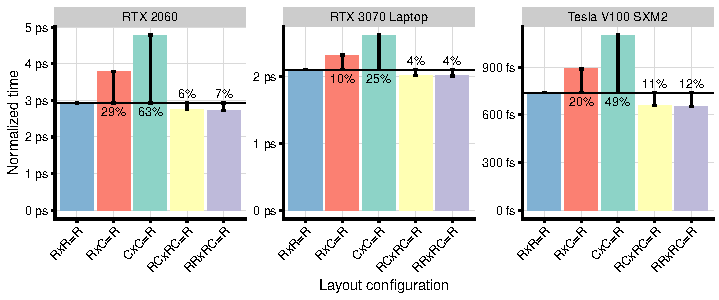
\includegraphics{noarr/plots/matmul_selected.pdf}
    \caption{Speedups of selected layout combinations relative to (row-major) baseline}
    \label{fig:matmul_speedup}
\end{figure}

The result verified that \textbf{RC} is superior to the baseline row-major layout in both input positions. Furthermore, the $R\times C=R$ configuration (often praised on sequential architectures) exhibits worse than the baseline on massively parallel hardware. While this was expected, the primary outcome of this benchmark is methodological: A selection of input and output layouts can be tested systematically without reimplementation effort, while the larger exploration size of the selection (enabled by low coding overhead) provides a solid guarantee that the best-identified solution is indeed a good choice for a high-performance software.


% -----------------------------------------------------------------------------
\subsection{Transformations}\label{sec:transformations}
% -----------------------------------------------------------------------------

The layout-agnostic algorithms can benefit from performance gains achieved by choosing the best layout for a given problem configuration and architecture. However, in real-world scenarios, the layout of the input and output data structures is often prescribed as an inherent part of the algorithm interface or selected by the caller (in the case of generic interfaces).

If the algorithm is complex enough and the performance gap between the prescribed layouts and optimal layouts is high, the data structures may be copied and transformed into their optimally organized counterparts to speed up the algorithm. With \Noarr{}, the transformation can be handled in a generic way. Following our examples with matrices, Listing~\ref{lst:transform} presents the central part of a generic transformer for 2D structures.

\begin{listing}
    \vspace{-10pt}
    \inputmintedcpp{noarr/code-snippets/transform-short.cpp}
    \vspace{-20pt}
    \caption{Key part of transformation routine for 2-index (2D) arrays}
    \label{lst:transform}
\end{listing}

In fact, we are currently extending \Noarr{} to handle the transformations in a generic way for any-dimensional structures, and we are exploring techniques how to select the best way of iterating the structures (e.g., selecting the best ordering of nested loops) in order to optimize memory transfers and caching. However, this research is well beyond the scope of this paper.


\subsubsection{Transformation overhead assessment.}

Employing transformations may be beneficial only under specific circumstances. Simply put, the algorithm must save more execution time than how long it takes to transform all the necessary data. We want to demonstrate the overhead assessment on the previously introduced matrix multiplication example.

We have analyzed the layout transformation overhead for various matrix sizes and layouts. The key results are summarized in Figure~\ref{fig:matmul_comp}. We have observed that in the case of larger matrices ($N>10,000$), the overhead is negligible, primarily because of the asymptotic complexity difference between the transformation algorithm ($\mathcal{O}(N^2)$) and the multiplication ($\mathcal{O}(N^3)$). For smaller matrices (with $N$ around $1000$), the relative ratio of the transformation to computation time expectably increased, and the transformation overhead caused the baseline to perform the best.

\begin{figure}
    \centering
    \includegraphics{noarr/plots/matmul_transform.pdf}
    \caption{Layout transformation times compared to actual matrix multiplication times}
    \label{fig:matmul_comp}
\end{figure}

As demonstrated, deciding whether or when a layout transformation can be beneficial may be complicated; however, with \Noarr{}, both the experiments and the actual decision to apply or not to the transformation can be implemented very quickly.

% Finally, it is worth mentioning that the overhead of the transform algorithm can be reduced by selecting an appropriate copy-ordering for different layouts. The example in Listing~\ref{lst:transform} is designed as optimal for row-major layout, but it may not be optimal for other types of transforms. One of the objectives for the future research is to extract meta-information from the layout structures that would allow us to automatically select the optimal transform strategy (e.g., ordering of the nested for-loops).

% \section{Layout Transformations}\label{sec:transformations}

The layout-agnostic algorithms can benefit from performance gains that are achieved by choosing the best layout for given problem and architecture. However, in real-world scenarios, the layout of the input and output data structures is often prescribed as an inherent part of the algorithm interface, or even selected by the caller (in case of generic interfaces). Here, we show a straightforward way to generate code that transforms the code into the desired layout.


% -----------------------------------------------------------------------------
\subsection{Semi-automated transformation layer}
% -----------------------------------------------------------------------------

An abstract workflow of any data-processing program may be simplified to 3 phases --- \emph{loading} of the data into possible intermediate structures, \emph{execution} of the operation on the data, and \emph{storing} of the contents of possible intermediate structures into the target buffers.

To ensure optimal layout for the execution while keeping the input and output format as prescribed or selected by the caller, an adaptive layer can be introduced between steps 1--2, and 2--3 of the workflow. This layer would handle the transformation of the data from the original `external' input format into the optimal `internal` input format, and from optimal output format to the final output format. Assuming that the memory management in the second step is properly decoupled from array representation, the \emph{layout transformation} in the adaptive layers can be written as a generic routine using \Noarr{} library, as shown on an example for arrays with 2 indexes in Listing~\ref{lst:transform}.

\begin{listing}
    \vspace{-10pt}
    \inputmintedcpp{noarr/code-snippets/transform.cpp}
    \vspace{-20pt}
    \caption{Generic layout transformation routine for 2-index arrays.}
    \label{lst:transform}
\end{listing}

In the example, the transformation function (lines 1--7) operates on two \texttt{bag} structures, copying their contents element by element from a bag with data that use input layout to a bag with the desired layout, effectively performing the layout transformation. A helper function (lines 9--20) further simplifies the data transformation by determining if a layout change is really needed, and executing transformation (and copying the data) conditionally only in that case.

\begin{listing}
    \vspace{-10pt}
    \inputmintedcpp{noarr/code-snippets/matmul_transform.cpp}
    \vspace{-20pt}
    \caption{Outline of layout transformation layer for matrix multiplication example.}
    \label{lst:matmul_transform}
\end{listing}

These transformation routines may be readily used in other algorithms, as demonstrated in Listing~\ref{lst:matmul_transform} that wraps a matrix multiplication algorithm similar to the one from Listing~\ref{lst:matmul}.

We note that it is possible to implement the layout transformation function generically for any layout, for example by adapting the layout objects to work in range-based for-loops. Complex design considerations of the implementation (especially the static forwarding of the dimension identifiers) are however out of scope of the current \Noarr{} implementation.

% -----------------------------------------------------------------------------
\subsection{Exploring all layout combinations}
% -----------------------------------------------------------------------------

Given the possibility to work with arbitrary input and output layouts, we may expand the experiment from Section~\ref{sec:layouts-agnostic} to a larger spectrum of possible combinations of input and output layouts. We utilize the schema from Listing~\ref{lst:matmul_transform} to systematically loop through and benchmark all $6^3$ combinations of the layouts for the tiled matrix multiplication. The results are shown in Figure~\ref{fig:matmul_heatmap_all}.

\begin{figure}
	\centering
	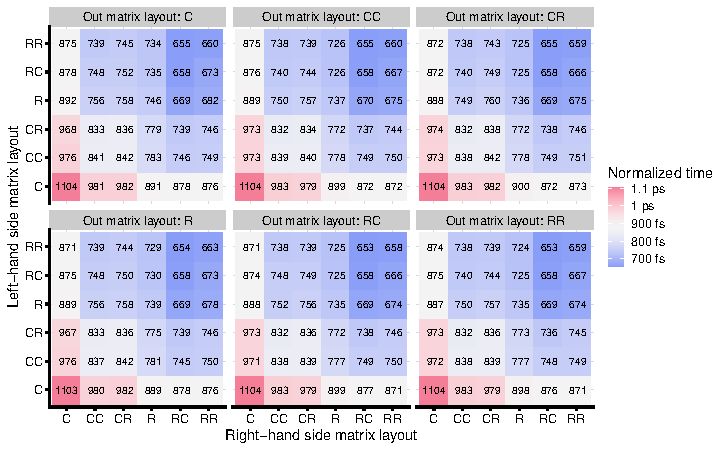
\includegraphics{plots/heatmap_all.pdf}
	\caption{Performance overview of layout combinations in matrix multiplication (X and Y axes represent the layout of right and left operand of the multiplication, layouts of the output are plotted separately). We report the normalized time per asymptotic operation, i.e., wall time divided by $N^3$.}
	\label{fig:matmul_heatmap_all}
\end{figure}

The results imply that the kernel performed best with $\textbf{RR}\times \textbf{RC}=\textbf{RR}$ layout combination, which was expected for tiled algorithm. The layout of input matrices turns out to be very important as the worst configuration ($\textbf{C}\times \textbf{C}$) is almost two times slower than the best one. On the other hand, the performance differences for the output matrix layouts are almost negligible. As in Section~\ref{sec:layouts-agnostic}, the main result is again methodological: The programmers may easily screen through all possible layouts for their data structures, and choose a reliable optimum for inclusion in production software.

% -----------------------------------------------------------------------------
\subsection{Transformation overhead}
% -----------------------------------------------------------------------------

While the algorithm performance is determined mainly by the layout combinations, the absolute performance differences are not huge. For example, the commonly used row-major format (i.e., $\textbf{R}\times \textbf{R} = \textbf{R}$) is only about 12\% slower on selected matrix sizes, which makes it at least competitive. We may therefore ask whether the data transformation overhead would not nullify the benefits of optimal layouts.

% The findings of this semi-automated layout transformation can in reasonably simple programmatic way show insights into the behavior of the specific function in terms of the memory access pattern and caches utilization. With minimal effort, this principle can be applied on multi-stage pipeline algorithms where each stage expects different memory layout for the most optimal computation. 

% However, a duration of the actual transformation needs to be accounted into as well. Depending on the layout pair to be transformed, the size of data and the actionable function, the duration of the transformation can sometimes diminish the performance gain resulted from the optimal layout usage in the selected algorithm. 

To clarify this concern, we have analyzed the layout transformation overhead for various matrix sizes and layouts. The key results are summarized in Figure~\ref{fig:matmul_comp}. We have observed that in the case of larger matrices ($N>10000$), the overhead is negligible, mostly because the asymptotic complexity difference between the transformation algorithm ($\mathcal{O}(N^2)$) and the multiplication ($\mathcal{O}(N^3)$). For smaller matrices (with $N$ around $1000$), the relative ratio of the transformation to computation time expectably increased. (Additionally, smaller matrices benefited more from caches, which make their layout slightly less important.) At that point, the baseline configuration $\textbf{R}\times\textbf{R}=\textbf{R}$ becomes the best option simply because it lacks the transformation overhead.

\begin{figure}
	\centering
	\includegraphics{plots/matmul_transform.pdf}
	\caption{Overhead of the layout transformation compared to actual time spent in the matrix multiplication algorithm. Only selected combinations of the layouts are shown for small and big matrix sizes.}
	\label{fig:matmul_comp}
\end{figure}

Finally, it is worth mentioning that the overhead of the transform algorithm can be reduced by selecting an appropriate copy-ordering for different layouts. The example in Listing~\ref{lst:transform} is designed as optimal for row-major layout, but it may not be optimal for other types of transforms. One of the objectives for the future research is to extract meta-information from the layout structures that would allow us to automatically select the optimal transform strategy (e.g., ordering of the nested for-loops).

\section{Performance Impact of Constant Expressions}\label{sec:perf}

One of the essential features of \Noarr{} is that the first-class structures propagate along with their templated types, allowing us to embed statically defined properties (most importantly, the constant dimensions of the structure) into the type itself. Therefore, the compiler can employ optimizations like compile-time evaluation of constant expressions or exact-sized loop unrolling, which might lead to more efficient execution or even automated vectorization. These optimizations rarely produce a game-changing improvement in performance; thus, the programmers often overlook them. However, utilization of \Noarr{} structure will introduce them naturally so the result code could run faster without any additional effort whilst maintaining other benefits like memory allocation decoupling or coding in a layout-agnostic manner.

To present the main idea, let us have an array $A$ of $N$ vectors in $\mathbb{R}^D$ where $N$ is a variable, and $D$ is a constant\footnote{If the code needs to handle several different dimensionalities $D$, it will be compiled for each $D$ independently thanks to the power of C++ templates.}. We want to compute the Euclidean distance between every vector in the array and given vector $q$ (e.g., to find $k$ nearest vectors, which is quite a typical task in many data-processing problems):

\begin{minted}[fontsize=\scriptsize]{c++}
  for (size_t i = 0; i < N; ++i) {
    float dist = 0.0f;
    for (size_t d = 0; d < D; ++d) {
      float diff = A[i*D + d] - q[d];
      dist += diff * diff;
    }
    dist = std::sqrtf(dist); // ...
  }
\end{minted}

When $D$ is a constant, the compiler could unroll the loop entirely without additional branches. It might even attempt to unroll the outer loop if $D$ is sufficiently small. The speedup achieved by having constant $D$ may easily reach factor $3\times$ for very small values of $D$ (e.g., $D=2$)\footnote{If we measure only the Euclidean distance computation.}.


% -----------------------------------------------------------------------------
\subsection{Indexing performance}
% -----------------------------------------------------------------------------

To demonstrate the impact of \Noarr{} structures, we have selected a 3D stencil problem as an example. Stencil is a simple function computed iteratively for every element of a regular grid. We have used an averaging stencil executed on a 3D grid which could be used as an approximative simulation of gas diffusion, for instance. Our objective is to emphasize the difference between situations when the grid dimensions are constant (at compile time) and when they are determined at runtime.

The main code of the stencil is in Listing~\ref{lst:stencil_base}. Run-time variables \texttt{size\_x}, \texttt{size\_y}, and \texttt{size\_z} denote the dimensions of the cube. The first part of this experiment aims at exposing only the compile-time optimizations of index computations, so we ensure that no optimizations related to constant dimensions are performed. Please note that the loops do not visit points residing on the faces of the grid so that we can ignore the border cases of the stencil function; thus, there are no branches in the code which leads to simpler and more stable measurement. 

\begin{listing}[h]
    \vspace{-10pt}
    \inputmintedcpp{noarr/code-snippets/stencil_base.cpp}
    \vspace{-20pt}
    \caption{Main stencil for-loop}
    \label{lst:stencil_base}
\end{listing}

A na\"{i}ve C-like implementation of the internal \texttt{stencil} function is presented in Listing \ref{lst:stencil_trivial}. It uses the same variables in the loop to index the data pointers, preventing the compiler from doing more elaborate compile-time optimizations. This code is used as a baseline for the performance comparison.

\begin{listing}[h]
    \vspace{-10pt}
    \inputmintedcpp{noarr/code-snippets/stencil_trivial.cpp}
    \vspace{-20pt}
    \caption{Na\"{i}ve implementation of stencil function}
    \label{lst:stencil_trivial}
\end{listing}
\vspace{-10pt}

Making the dimensions constant may help the compiler to generate more optimal code. In C++, this can be achieved simply by defining the \texttt{size\_*} variables as \texttt{constexpr}; however, such constants need to be declared at the global level, which significantly undermines any encapsulation or reusability of the code. Better way is to use fix-sized containers like \texttt{std::array} and make the stencil code templated so it can be used with any compatible containers (including \texttt{std::vector}).

\begin{listing}[h]
  \vspace{-10pt}
  \inputmintedcpp{noarr/code-snippets/stencil_noarr.cpp}
  \vspace{-20pt}
  \caption{\Noarr{} implementation of stencil with constant-sized \texttt{array}}
  \label{lst:stencil_noarr}
\end{listing}
\vspace{-10pt}

\Noarr{} provides a fixed layout structure \texttt{array}, which fulfills a similar role, but it can be easily integrated into more complex nested structures (even with custom layouts). Listing \ref{lst:stencil_noarr} presents the internal \texttt{stencil} rewritten for \Noarr{}. The dimensions of the grid are no longer passed as variables, but they are embedded in the type of the \texttt{bag} structure as constants. Line $1$ shows the assembling of the layout structure using a predefined \texttt{array} template.

To evaluate the performance, we have selected a grid of a specific size ($2^{20} \times 32 \times 32$) which confines the meaning of the diffuse simulation for a specific environment (e.g., gas in a pipe). The main reason is that the performance improvement caused by the compile-time optimizations is difficult to measure on regular structures since it takes only a small portion of overall time (especially when the computation causes many cache misses). This shape requires more index computations relative to other operations, making the difference more pronounced in the measurements.

\begin{figure}[h]
  \vspace{-10pt}
	\centering
	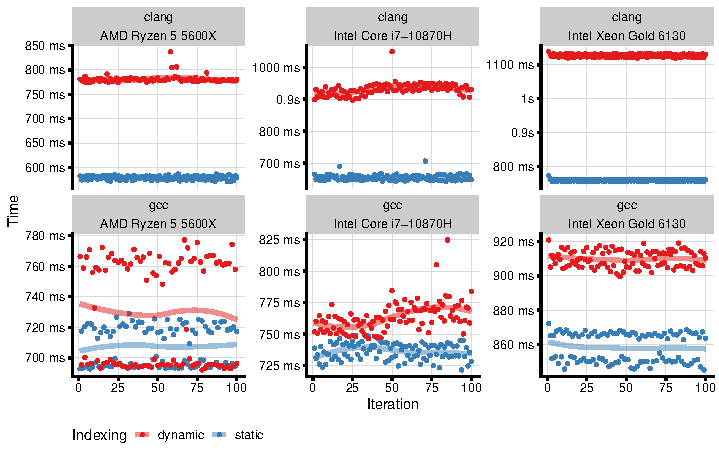
\includegraphics{noarr/plots/stencil.pdf}
	\caption{Wall times of $100$ stencil iterations (plotted lines represent the local regression of the measured times)}
	\label{fig:stencil}
  \vspace{-10pt}
\end{figure}

Figure \ref{fig:stencil} shows the comparison results of the two presented stencil implementations on three platforms using two compilers. The benefits of compile-time optimizations are visible on every platform and with both tested compilers, albeit there is only a small difference in some configurations. The details regarding the experimental methodology are summarized in Appendix~\ref{appendix:methodology}.


% -----------------------------------------------------------------------------
\subsection{Constant-loops optimizations}
% -----------------------------------------------------------------------------

The second part of this experiment extends the compile-time optimizations to the nested stencil grid loops. It requires replacing \texttt{size\_*} variables in the main loops (Listing \ref{lst:stencil_base}) with constants (i.e., \texttt{constexpr} or template arguments) so the compiler has enough information to perform exact loop-unrolling and better vectorization-related optimizations.

\begin{listing}[h]
  \vspace{-10pt}
  \inputmintedcpp{noarr/code-snippets/stencil_base_bag.cpp}
  \vspace{-20pt}
  \caption{Updated stencil for-loop with \texttt{bag} structure}
  \label{lst:stencil_base_bag}
\end{listing}
\vspace{-10pt}

However, converting these variables to constants may be quite tedious, especially if we want the code to be generic for both constant and non-constant scenarios. This particular issue can be easily overcome by utilization of \Noarr{} \texttt{bag} structures. Having the layout information encoded both in the structure type and the object, method \texttt{get\_length} can query dimension sizes and returns a constant or variable based on the layout specification, all this being decided at compile time. The grid loop function from Listing \ref{lst:stencil_base} needs to be rewritten as demonstrated in Listing~\ref{lst:stencil_base_bag}.

\begin{figure}[H]
  \vspace{-10pt}
	\centering
	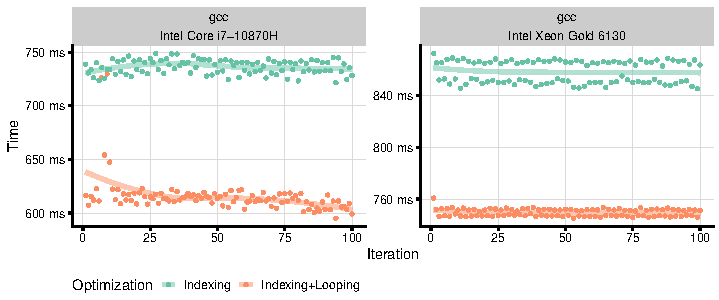
\includegraphics{noarr/plots/stencil_loop.pdf}
	\caption{Stencil execution times of two optimizations --- compile-time \emph{indexing} and the addition of constant-induced loop unrolling (\emph{indexing+looping})}
	\label{fig:stencil_wloop}
  \vspace{-10pt}
\end{figure}

Figure \ref{fig:stencil_wloop} presents the performance improvements of exposing constant variables to the grid iteration loop. We have included only measurements of programs compiled by \texttt{gcc} since \texttt{clang} was not able to take advantage of the constant values when they are passed through the \texttt{bag} structure interface.

\section{Implementation and Technical Insights}\label{sec:implementation}

The \Noarr{} library\footnote{\url{https://github.com/ParaCoToUl/noarr-structures}} is logically divided into three levels, each building on top of the previous one: \emph{structures}, \emph{functions}, and \emph{object wrappers}. The first two layers provide a rather low-level functional approach, while the last one encapsulates the first two into a more traditional C++ object-oriented design.

% -----------------------------------------------------------------------------
\subsection{Structures} 
% -----------------------------------------------------------------------------

A \emph{structure} is an object that stores information about a data layout. It exposes the information via a~simple interface, providing its size in bytes (\texttt{size()}), the range of indices it supports (\texttt{length()}) and a current offset from the beginning of the structure in bytes (\texttt{offset()}).

The most trivial structure is \texttt{scalar} (Listing \ref{lst:scalar}), which wraps the `base' values to be used in more complex layouts. Scalar often wraps simple types like \texttt{float}, but it can also wrap any fixed-size C++ type (such as \texttt{struct} or \texttt{std::tuple}). The methods \texttt{length()} and \texttt{offset()} of \texttt{scalar} always return $0$ because \texttt{scalar} represents only a single element.

\begin{listing}[h]
  \vspace{-10pt}
  \inputmintedcpp{noarr/code-snippets/scalar.cpp}
  \vspace{-20pt}
  \caption{A core part of the \texttt{scalar} structure used for wrapping simple values}
  \label{lst:scalar}
\end{listing}

The \texttt{array} structure (Listing \ref{lst:array}) is more complicated: Like \texttt{std::array}, it represents a~fixed-size array with a named dimension and statically defined number of elements of a given \emph{substructure}~type. Unlike \texttt{scalar} which wraps a \emph{trivial type}, \texttt{array} is contains a \Noarr{} \emph{structural type}.

An important aspect of the structures is their ability to be combined and nested to create a \emph{structure tree}. For instance, the composition of \texttt{scalar} and \texttt{array} is quite straightforward:
\begin{itemize}
\item\mintinline[fontsize=\scriptsize]{c++}{array<'a', 10, scalar<float>>}
defines an array of $10$ \texttt{float}s,
\item\mintinline[fontsize=\scriptsize]{c++}{array<'i', 4, array<'j', 8, scalar<int>>>}
represents a~$4\times8$ row-major integer matrix layout,
\item\sloppy\mintinline[fontsize=\scriptsize]{c++}{array<'j', 8, array<'i', 4, scalar<int>>>}
represents the same matrix in a column-major layout.
\end{itemize}

\begin{listing}[h]
  \vspace{-10pt}
  \inputmintedcpp{noarr/code-snippets/array.cpp}
  \vspace{-20pt}
  \caption{\Noarr{} \texttt{array} structure (some methods are omitted for brevity)}
  \label{lst:array}
\end{listing}

All structures inherit from class \texttt{contain}, which has several purposes: It serves as recursive storage for the wrapped structure, holds some useful meta-information about the nested substructures, and stores possible additional data for the structure, such as dynamic dimension length or the current offset index. Querying for various properties, which is its main purpose, is demonstrated in Listing \ref{lst:array}. The \texttt{array} implements the \texttt{size()} function using the information (size) from its immediate substructure (line $4$). In the example, queries work recursively on subsequent immediate substructures until the recursion is halted in \texttt{scalar::size()}. Using this mechanism, \texttt{contain} allows us to create the nested hierarchy of the structure tree easily.

There are several other built-in structures in \Noarr{} library, such as \texttt{vector} and \texttt{tuple} (analogical to \texttt{std::vector} and \texttt{std::tuple}), which provide sufficient arsenal for composing memory layouts of many regular-shaped data structures. Moreover, the library design makes it open for extensions, and programmers may implement additional custom layout structures.


% -----------------------------------------------------------------------------
\subsection{Functions}
% -----------------------------------------------------------------------------

\Noarr{} \emph{functions} are C++ \mintinline{c++}{constexpr} functions that serve as an expressive tool for obtaining complex information from the structure trees. They are used to compute offsets for memory pointers to provide indexation, transform structures, and query dimension lengths using a single, extensible functional interface.

Calling function \texttt{f} on a structure \texttt{s} is achieved using the (overloaded) `pipe' operator \texttt{|}. Expression \texttt{s | f} denotes that \texttt{f} is applied on \texttt{s} (note this may sometimes differ from \texttt{f(s)} as detailed later in this section).

For example, the function \texttt{get\_length()} traverses structure tree and calls \texttt{length()} on a substructure with the given dimension name:
\begin{minted}[fontsize=\scriptsize]{c++}
  size_t i_len = a_structure | get_lenght<'i'>();
\end{minted}

The function \texttt{set\_length()} proceeds similarly, but when a matching substructure is found, the whole structure is reconstructed to carry the new length. The following example shows that functions can be additionally chained one after another. Notably, all structures are immutable, which allowed us to ensure that \texttt{unsized\_s} does not carry any unnecessary data:
\begin{minted}[fontsize=\scriptsize]{c++}
  auto unsized_s = vector<'i', vector<'j', scalar<float>>>();
  auto sized_s = unsized_s | set_length<'i'>(4) | set_length<'j'>(8);
\end{minted}

A function application on a structure may fail, such as when querying a~length of a non-existing dimension. We say the function is \emph{not applicable} on a~structure. Taking the aforementioned two functions into account and the fact that every structure forms a structure tree, it is possible that a~function is not \emph{directly applicable} on the topmost structure but is applicable on some structures in the structure tree. For this reason, we distinguish three \emph{piping mechanisms} that govern different means of the function-structure application:

\begin{itemize}
    \item \emph{Top application} (or \emph{direct application}). This is the simplest form of piping, where \texttt{s | f} is equivalent to \texttt{f(s)}. In other words, the function is applied directly to the topmost structure. 
    \item \emph{Get application}. Given the piping \texttt{s | f}, if \texttt{f(s)} is not applicable the piping mechanism attempts to apply \texttt{f} to the substructures of \texttt{s} recursively. It fails if \texttt{f} does not apply to any of the substructures or if it applies to more substructures. The trivial representative being \texttt{get\_length()}, because there should be exactly one node in a structure tree with a specified dimension.   
    \item \emph{Transform application}. \texttt{s | f} either results in top application when \texttt{f(s)} is applicable or \texttt{f} is transformatively applied on all \emph{direct} substructures of \texttt{s}. If the latter, the structure is reconstructed with these changes to the substructures. 
\end{itemize}

The piping mechanism is implemented using C++ \mintinline{c++}{constexpr} functions and metaprogramming. Together with the static nature of substructure hierarchies that encompasses the structure layer, the implementation is very efficient since it provides the necessary space for compiler optimizations. We can demonstrate this by precisely describing the operations executed when a function with the get application is applied to a structure. Let us have the following structure and function:
\begin{minted}[fontsize=\scriptsize]{c++}
  auto v4 = vector<'a', vector<'b', vector<'c', vector<'d', scalar<int>>>>>();
  auto f = get_length<'d'>();
\end{minted}
Expression \texttt{v4 | f} must perform a traversal of the structure tree to find the matching dimension. Fortunately, the way the structures and functions are implemented ensures that there is no run-time loop in the implementation. Because all substructures are known in compile-time, the traversal loop is unrolled using metaprogramming techniques. Furthermore, because the values are also known at compile-time, the result can be partially evaluated and, in turn, \emph{no run-time code is generated}. In summary, applying \texttt{v4 | f} produces four unrolled function applications, three of which produce no operation at all (and usually get discarded by a compiler), and only one results in calling \texttt{length()} on a~substructure that can be evaluated by the compiler.


% -----------------------------------------------------------------------------
\subsection{Object wrappers} 
% -----------------------------------------------------------------------------

Object wrappers provide object-oriented management of structures, functions, and the actual data. \Noarr{} library offers two kinds of such objects --- structure \emph{wrappers} and \texttt{bags}.

A \texttt{wrapper} simplifies the work with structures by bundling the applications of the most common \Noarr{} functions into member methods. That way, with a wrapper \texttt{w} of a structure \texttt{s} we can directly write \mintinline{c++}{w.get_length<'d'>()} instead of \mintinline{c++}{s | get_length<'d'>()}.

A \texttt{bag} provides the same interface as a~\texttt{wrapper} but also contains a pointer to the underlying memory. To work with the data, it implements a~member method \mintinline{c++}{at<Dims...>(idxs...)} that is used to index the data pointer with respect to the enveloping structure layout. This method is a wrapper for the library function \texttt{get\_at}. Without using a \texttt{bag}, the indexing might look like this:
\begin{minted}[fontsize=\scriptsize]{c++}
  auto s = array<'j', 8, array<'i', 4, scalar<float>>>();
  float* ptr = allocate_memory_bytes(s.size());
  float x = s | get_at<'i', 'j'>(ptr, 2, 3);
\end{minted}
The \texttt{bag} binds the layout together with data, systematizing the computation on the last line as follows:
\begin{minted}[fontsize=\scriptsize]{c++}
  auto b = bag(s, ptr);
  float x = b.at<'i', 'j'>(2, 3);
\end{minted}

Furthermore, to manage an explicitly bound external pointer, \texttt{bag} can also allocate the underlying memory automatically if no pointer is given (i.e., it also carries the semantics of a smart pointer). Technically, \texttt{bag} can belong to either one of two semantic groups according to the way it acquires data:
\begin{itemize}
    \item \emph{Owning semantics.} The bag is constructed only with a structure to envelop. The data pointer of exact length is automatically allocated using standard memory management (e.g., by \texttt{unique\_ptr}), and the length is determined by calling \texttt{size()} on the wrapped structure.
    \item \emph{Borrowing semantics.} The bag is constructed with both structure and data pointer. In this case, the deallocation, as well as ensuring the proper data-block length, has to be enforced by the caller.
\end{itemize}



% \begin{enumerate}
%     \item \emph{Structures} --- .
%     \item \emph{Functions} --- C++ pure constexpr functions that serve as an expressive tool to obtain complex information from a tree of structures.
%     \item \emph{Object wrappers} --- Classes that provide object oriented wrappers on top of the previous layers.
% \end{enumerate}

% \Noarr{} library distinguishes three objects:
% \begin{itemize}
%     \item \texttt{Structure} A small, tree-like object, that represents the structure of the data. It does not contain the data itself, nor a pointer to the data. It can be thought of as a function that maps indices to memory offsets (in bytes). It stores information, such as data dimensions and tuple types.
%     \item \texttt{Data} A continuous block of bytes that contains the actual data. Its structure is defined by a corresponding Structure object.
%     \item \texttt{Bag} Wrapper object, which combines structure and data together.
% \end{itemize}

% \subsection{Structure}

% Supported layouts:
% \begin{itemize}
%     \item \texttt{Containers} Vector or array. 
%     \item \texttt{Scalars} int, float, size\_t.
%     \item \texttt{Tuples} Ordered set of previous two.
% \end{itemize}

% \subsection{Functions}

% Means of modifying structures and applying them on data.

% \begin{itemize}
%     \item \texttt{get\_length get\_offset} ... read
%     \item \texttt{set\_length, fix} ... modify  
%     \item \texttt{get\_at} ... index
% \end{itemize}

% \subsection{Internal representation}

% Thx to majority of logic is in functions, actual layout structure is very simple.

% implemented as a tree of sub structures ... easily extensible ... show simple example (reverse vector)

% \subsection{Data and Bag}

% Data must be continuous (no jagged).

% Bag acquires data 2 ways:
% \begin{itemize}
%     \item \emph{borrowing semantics} gets data via pointer as constructor param
%     \item \emph{owning semantics} allocates data using standard memory management
% \end{itemize}



% nasledujici text je zkopirovan z paper.tex (brainstorming), bure potreba to jeste poradne rozmyslet (aby tahle sekce nebyla moc tlusta, ale byla vystizna); rozhodne to nema byt reference kodu
% (quick peek on the most important structures + how they are implemented, this must not look like a reference)

% 1. built-in struktury vector, array, scalar, tuple
% 2. ako sa s nimi pracuje: bag, set\_length, indexovanie, structure wrapper
% 3. impl. details?

% \section{Flexible data layout}

% 1. noarr je plne rozsiritelny na definovanie vlastneho layoutu. ukazat na jednoduchom priklade
% ako sa to robi (reverse-vector/matrix napr.)
% 1.1. vysvetlit noarr::compose <=> std::tuple
% 1.2. vysvetlit vyznam preco vsetko je constexpr  
% 2. na vacsom priklade ukazat predosle body (cache aware layout na matmul v CUDE) + porovnat s trivial impl

% \section{Easy switch between layouts in noarr workflows}

% 1. ukazat, ze noarr sturktury su vo funkcii/kerneli zamenne
% 2. ukazat moznost jednoduchej transformacie medzi layoutmi
% 2.1. ukazat funckie na vlozenie transformacnej vrstvy do algoritmu
% 3. na vacsom priklade ukazat predosle body - full-blown aplikacia transformacnych vrstiev + layoutingu (porovnat wall time [i s transformaciou] oproti algoritmu s trivialnym layoutom)

\section{Related Work}\label{sec:relwork}

A significant group of works that touch the problem of memory layouts are parallel programming languages such as X10~\cite{charles2005x10}, Chapel~\cite{chamberlain2007parallel} or Legion~\cite{bauer2012legion}. Apart from providing syntax for simple parallel code expression, these languages allow for data decomposition into regions that can be mapped within the same memory space or more complex non-uniform memory spaces. Hence, the memory layout expression addressed by these works is only researched to the point of high-level data distribution among processing elements.

Application-specific library generators, or \emph{active libraries}, also utilize memory layouts. The most known representatives are ATLAS~\cite{whaley1998automatically}, SPIRAL~\cite{puschel2004spiral} and FFTW~\cite{frigo1998fftw} specializing in linear algebra, signal processing, and Fast Fourier Transform, respectively. They are trying to mitigate portability issues of manually optimized programs by selecting the best interprocedural optimizations for the hosting system using autotuning. Usually, these optimization strategies include some form of memory layout selection. It is important to note that active libraries target different stages in programming than \Noarr{}; rather than performing the layout selection from the hardcoded set of layouts, \Noarr{} provides means to \emph{implement} such layout selections in a more extensible and object-oriented way.

The most related works we found are Kokkos \cite{9485033}, and GridTools \cite{AFANASYEV2021100707}. These libraries allow the coupling of arbitrary data structures with memory layouts which can be either selected from a set of predefined layouts or programmatically customized.

GridTools specialize in block-structured grid applications such as combustion, seismic, and weather simulations, working with generalized stencil-like patterns. The library defines a storage infrastructure component that controls the layout, alignment, and padding of stored data fields. A layout is specified in code at compile time by selecting one of the predefined target backends, each well suited for a specific use case, such as vector instructions or GPU kernels. The library can be extended with new programmer-specified backends, but the layout can be altered only by permuting dimension order in a regular $n$-dimensional array. 

An interesting approach is taken in the Kokkos library, which specifies the \texttt{View} class that couples the definition of data memory space, allocation, and layout altogether using C++ policy classes, yielding an object of similar functionality as our \texttt{bag}. The memory resource and allocation mechanism are abstracted and defined by the template argument. Kokkos provides multiple memory spaces such as \texttt{HostSpace}, \texttt{CudaSpace}, \texttt{CudaHostPinnedSpace}, thus representing CPU and GPU physical memory and their combinations.

In Kokkos, the memory layout is either implicitly deduced from the memory space or explicitly specified as another template parameter. The library implements row and column-major layouts together with the layout with strides with custom sizes. Kokkos allows user-defined memory layouts by defining a new layout policy and implementing a function that defines a bijective mapping between index space and memory addresses. However, this mapping must be defined on a regular $n$-dimensional array, using a minimal API that fits the \texttt{View} class.

Language-wise, our approach is similar to (and inspired by) known concepts from functional programming. Materialized, first-class composable references to sub-structures uncoupled from data have been extensively studied as optics~\cite{foster2007combinators}. In particular, the internal structures that implement the selection of array slices at certain indexes are similar to the concept of indexed lenses --- kind of references that transparently provide information about the current index in a complicated structure, as summarized by Clarke et~al.~\cite{clarke2020profunctor} In the future, it might be interesting to examine whether more advanced optics may be modeled in C++ for array accesses, e.g., expressing repeated data accesses similarly to lens-based traversals or reconstructing the user-facing indexes from known offsets using isomorphisms.


% TiDa and GridTools specialize in block-structured grid applications such as combustion, seismic, and weather simulations, working with generalized stencil-like patterns. TiDa allows the programmer to express data locality and layout at the array construction by declaring how the data is divided into regions to be accessed by different processing elements (such as NUMA nodes), which are further divided into tiles for finer layout granularity.


% Extensive research has been performed in choosing optimal layouts concerning a provided algorithm. For example, Sharma et al.~\cite{10.1145/2747875} investigated a transformation technique called array interleaving, which combines the storage of data elements from multiple arrays to achieve better data locality. Sung et al.~\cite{sung2010data} presented compiler optimization that enables data layout transformation for structured grid codes with dynamically allocated arrays (e.g., stencil functions). These involve source-to-source program transformation to generate functions that can transform the data into a `better' layout with more locality. Both authors observed performance increases, reductions in memory transfers, and improvements in memory access patterns.


% parallel libraries with much wider functionalities than just layout transformations:
% \begin{enumerate}
%     \item \emph{kokkos} \cite{9485033,CARTEREDWARDS20143202}
%     \subitem provides class View that defines memory space, allocation, layout alltogether via policy classes.
%     \subitem Memory space template represents allocation mechanism. Kokkos imlpements multiple types: HostSpace, CudaSpace, CudaHostPinnedSpace indexing is implemented by DeviceType, a policy class.
%     \subitem Layout is statically inlined, primarily LayoutLeft, LaoutRight, LayoutStride.
%     \subitem on top of that, there is third policy class. Memory Traits. Provides additional info about memory behavior --- whether to utilize texture memory in CUDA, atomic access, ...
%     \subitem View in its constructor defines sizes of dimensions, but can be provided staticaly via template argument as well. In its constructor, it allocates data according to memory space policy. It can be coppied to create a view of the data. effectively creating shared-ptr semantics over the data.
%     \item \emph{TiDa} \cite{tida}. library supports programs operating on block-structured grid applications such as combustion, seismic, weather simulations and image processing. Divides data into regions to improve data locality on NUMA nodes. regions are divided into tiles improve cache reuse.
%     \item \emph{GridTools} \cite{AFANASYEV2021100707}. Only custom possibility is to permute dimensions in ndarray. Other than that, it supports general layouts for some common cases (vectorization, gpu).
% \end{enumerate}

% works targeted on finding optimal memory layout and layout transformation:
% \begin{enumerate}
%     \item \cite{10.1145/2747875} efficient layout transformation via array interleaving to improve memory accesses for SIMD FUs, SMPs, vector registers. Achieves decrease in memory energy consumption 6-36 percent.
%     \item \cite{sung2010data} presents compiler optimization that enables data layout transformation for structured grid
%     codes (stencil, fluid dynamics, heat dicipation) in CUDA. It involves source to source compilation that generates transformative functions that result in layout with better data locality. The code must be further compiled by NVCC (or other suitable) compiler.   
% \end{enumerate}

% purely functional haskel libarary for writing multi-dimensional arrays.


% -----------------------------------------------------------------------------
\section{Conclusion}\label{sec:conclusion}
% -----------------------------------------------------------------------------

We have presented a new high-performance approach for managing the complexity of offset computation in array-like data structures in modern C++. We introduced first-class layout structures that can be used to describe complex array layouts and run the required offset computations. The implementation is based on C++ template metaprogramming, exposing a rich interface for manipulating the structures with index mnemonics while enabling many compiler optimizations by properly separating static compile-time parameters and known constants from dynamic data.

The technique promotes complete decoupling of array indexing from memory allocation, which makes it applicable for many scenarios, including direct processing of memory-mapped files or re-using the same data structure layout in various memory spaces (e.g., offloading computations to GPUs). We showed that the layout structures, combined with the C++ templating system, make it easier to create layout-agnostic algorithms and functions, leading to a simpler selection of optimal layouts for a given hardware platform and problem configuration. Additionally, the utilization of layout structures makes it easier to create semi-automated layout transform routines, which can improve the performance of many algorithms.

We have implemented the proposed ideas in \Noarr{}, a prototype library demonstrating the viability of the approach. We demonstrated the benefits in several examples and experiments; most importantly, we showcased the ability to write shorter program source code that promotes easier experimentation and compilation into faster solutions. The library is publicly available as an open-source portable to all mainstream compilers, including CUDA \texttt{nvcc}, and may be readily used in designing new libraries that consider performance a priority. We expect that the approach will simplify the research focusing on optimizations and automatic tuning of the performance of complex parallel algorithms.

% \subsection*{Acknowledgements}

% This work was supported by Charles University institutional funding SVV 260451.

% \appendix

\section{Experimental Methodology}\label{appendix:methodology}

The main objective of the benchmarking was to measure the speedups achieved by different layout combinations to support the claims mentioned in the work\footnote{More details and the data are in the replication package \url{https://github.com/asmelko/ica3pp22-artifact}.}. A more complex performance evaluation is beyond the scope of this paper and is planned in future work.

% -----------------------------------------------------------------------------
\subsection{GPU benchmarking setup}
% -----------------------------------------------------------------------------

In the results, we present mainly the kernel execution times measured by the high-precision system clock, which is available on all platforms. The relative standard deviations in $20$ collected measurements of each result were less than $5$\% of the mean value in all cases, so we report only the mean values.

Due to the page limit, the presented results were limited to matrices of sizes $(1008\times 1008)$ and $(10,080\times 10,080)$. However, more extensive testing on other problem instances, including a broader range of matrix sizes and non-square matrices, exhibited similar results.

The results were collected on the following platforms:
\begin{itemize}
    \item NVIDIA Tesla V100~SXM2 (Volta, CC 7.0, $1.3$GHz), Rocky Linux 8
    \item NVIDIA GeForce RTX 2060 (Turing, CC 7.6, $1.7$GHz), Windows 10
    \item NVIDIA GeForce RTX 3070 laptop (Ampere, CC 8.6, $1.6$GHz), Windows 11
\end{itemize}

All platforms used CUDA toolkit 11.6 with an up-to-date driver. These devices represent three of the most recent Nvidia architectures and three typical hardware platforms (server, desktop PC, and laptop). Hence, we claim that the measurements sufficiently represent contemporary CUDA-enabled GPUs.


% -----------------------------------------------------------------------------
\subsection{CPU benchmarking setup}
% -----------------------------------------------------------------------------

We ran the kernel in $100$ iterations for the stencil benchmark, plotted the local regression outlining the mean value, and distinguished the outliers.
The measurements were conducted using the following CPUs:
\begin{itemize}
    \item AMD Ryzen 5 5600X (hi-end desktop CPU, $3.70$GHz), Windows 10
    \item Intel Core i7-10870H (laptop CPU, $2.20$GHz), Windows 11
    \item Intel Xeon Gold 5218 (server CPU, $2.3$GHz), Rocky Linux 8.
\end{itemize}

Due to the fact that some compilers may optimize \texttt{constexpr} expressions better than others, we compiled the benchmark using \texttt{clang++} v$12$ and \texttt{g++} v$11$ compilers with \texttt{-03} flag.
We also compiled the stencil benchmark using the MSVC C++ compiler, but the results showed that it could not sufficiently optimize \Noarr{} code in the current version; hence, MSVC results are not included.

All benchmarking datasets were synthetic, with data sampled randomly from the same uniform distribution. We consider synthetic validation sufficient since the performance of the benchmarked algorithms is not data-dependent.




\chapter*{Conclusion}
\addcontentsline{toc}{chapter}{Conclusion}


%%% Bibliography
%%% Bibliography (literature used as a source)
%%%
%%% We employ bibTeX to construct the bibliography. It processes
%%% citations in the text (e.g., the \cite{...} macro) and looks up
%%% relevant entries in the bibliography.bib file.
%%%
%%% The \bibliographystyle command selects, which style will be used
%%% for references from the text. The argument in curly brackets is
%%% the name of the corresponding style file (*.bst). Both styles
%%% mentioned in this template are included in LaTeX distributions.

\bibliographystyle{plainnat}    %% Author (year)
% \bibliographystyle{unsrt}     %% [number]

\renewcommand{\bibname}{Bibliography}

%%% Generate the bibliography. Beware that if you cited no works,
%%% the empty list will be omitted completely.

\bibliography{bibliography}

%%% If case you prefer to write the bibliography manually (without bibTeX),
%%% you can use the following. Please follow the ISO 690 standard and
%%% citation conventions of your field of research.

% \begin{thebibliography}{99}
%
% \bibitem{lamport94}
%   {\sc Lamport,} Leslie.
%   \emph{\LaTeX: A Document Preparation System}.
%   2nd edition.
%   Massachusetts: Addison Wesley, 1994.
%   ISBN 0-201-52983-1.
%
% \end{thebibliography}


%%% Figures used in the thesis (consider if this is needed)
\listoffigures

%%% Tables used in the thesis (consider if this is needed)
%%% In mathematical theses, it could be better to move the list of tables to the beginning of the thesis.
\listoftables

%%% Abbreviations used in the thesis, if any, including their explanation
%%% In mathematical theses, it could be better to move the list of abbreviations to the beginning of the thesis.
\chapwithtoc{List of Abbreviations}

%%% Doctoral theses must contain a list of author's publications
\chapwithtoc{List of publications}

%%% Attachments to the doctoral thesis, if any. Each attachment must be
%%% referred to at least once from the text of the thesis. Attachments
%%% are numbered.
%%%
%%% The printed version should preferably contain attachments, which can be
%%% read (additional tables and charts, supplementary text, examples of
%%% program output, etc.). The electronic version is more suited for attachments
%%% which will likely be used in an electronic form rather than read (program
%%% source code, data files, interactive charts, etc.). Electronic attachments
%%% should be uploaded to SIS and optionally also included in the thesis on a~CD/DVD.
%%% Allowed file formats are specified in provision of the rector no. 72/2017.
\appendix
\chapter{Attachments}

\section{First Attachment}

\openright
\end{document}
